\documentclass[11pt,fleqn]{book} 
\usepackage[top=3cm,bottom=3cm,left=3.2cm,right=3.2cm,headsep=10pt,letterpaper]{geometry} 
\usepackage{xcolor}
\usepackage{url}
\definecolor{ocre}{RGB}{52,177,201} 
\usepackage{avant} 
\usepackage{mathptmx} 
\usepackage{microtype} 
\usepackage[utf8]{luainputenc}
\usepackage[T1]{fontenc} 
\usepackage[style=alphabetic,sorting=nyt,sortcites=true,autopunct=true,babel=hyphen,hyperref=true,abbreviate=false,backref=true,backend=biber]{biblatex}
\addbibresource{bibliography.bib} 
\defbibheading{bibempty}{}
\newcommand{\minuseq}{\mathrel{-}=}



%----------------------------------------------------------------------------------------
%	VARIOUS REQUIRED PACKAGES
%----------------------------------------------------------------------------------------

\usepackage{titlesec} % Allows customization of titles

\usepackage{graphicx} % Required for including pictures
\graphicspath{{Pictures/}} % Specifies the directory where pictures are stored

\usepackage{lipsum} % Inserts dummy text

\usepackage{tikz} % Required for drawing custom shapes

%\usepackage[english]{babel} % English language/hyphenation
\usepackage[german]{babel}

\usepackage{enumitem} % Customize lists
\setlist{nolistsep} % Reduce spacing between bullet points and numbered lists

\usepackage{booktabs} % Required for nicer horizontal rules in tables

\usepackage{eso-pic} % Required for specifying an image background in the title page

%----------------------------------------------------------------------------------------
%	MAIN TABLE OF CONTENTS
%----------------------------------------------------------------------------------------

\usepackage{titletoc} % Required for manipulating the table of contents

\contentsmargin{0cm} % Removes the default margin
% Chapter text styling
\titlecontents{chapter}[1.25cm] % Indentation
{\addvspace{15pt}\large\sffamily\bfseries} % Spacing and font options for chapters
{\color{ocre!60}\contentslabel[\Large\thecontentslabel]{1.25cm}\color{ocre}} % Chapter number
{}  
{\color{ocre!60}\normalsize\sffamily\bfseries\;\titlerule*[.5pc]{.}\;\thecontentspage} % Page number
% Section text styling
\titlecontents{section}[1.25cm] % Indentation
{\addvspace{5pt}\sffamily\bfseries} % Spacing and font options for sections
{\contentslabel[\thecontentslabel]{1.25cm}} % Section number
{}
{\sffamily\hfill\color{black}\thecontentspage} % Page number
[]
% Subsection text styling
\titlecontents{subsection}[1.25cm] % Indentation
{\addvspace{1pt}\sffamily\small} % Spacing and font options for subsections
{\contentslabel[\thecontentslabel]{1.25cm}} % Subsection number
{}
{\sffamily\;\titlerule*[.5pc]{.}\;\thecontentspage} % Page number
[] 

%----------------------------------------------------------------------------------------
%	MINI TABLE OF CONTENTS IN CHAPTER HEADS
%----------------------------------------------------------------------------------------

% Section text styling
\titlecontents{lsection}[0em] % Indendating
{\footnotesize\sffamily} % Font settings
{}
{}
{}

% Subsection text styling
\titlecontents{lsubsection}[.5em] % Indentation
{\normalfont\footnotesize\sffamily} % Font settings
{}
{}
{}
 
%----------------------------------------------------------------------------------------
%	PAGE HEADERS
%----------------------------------------------------------------------------------------

\usepackage{fancyhdr} % Required for header and footer configuration

\pagestyle{fancy}
\renewcommand{\chaptermark}[1]{\markboth{\sffamily\normalsize\bfseries\chaptername\ \thechapter.\ #1}{}} % Chapter text font settings
\renewcommand{\sectionmark}[1]{\markright{\sffamily\normalsize\thesection\hspace{5pt}#1}{}} % Section text font settings
\fancyhf{} \fancyhead[LE,RO]{\sffamily\normalsize\thepage} % Font setting for the page number in the header
\fancyhead[LO]{\rightmark} % Print the nearest section name on the left side of odd pages
\fancyhead[RE]{\leftmark} % Print the current chapter name on the right side of even pages
\renewcommand{\headrulewidth}{0.5pt} % Width of the rule under the header
\addtolength{\headheight}{2.5pt} % Increase the spacing around the header slightly
\renewcommand{\footrulewidth}{0pt} % Removes the rule in the footer
\fancypagestyle{plain}{\fancyhead{}\renewcommand{\headrulewidth}{0pt}} % Style for when a plain pagestyle is specified

% Removes the header from odd empty pages at the end of chapters
\makeatletter
\renewcommand{\cleardoublepage}{
\clearpage\ifodd\c@page\else
\hbox{}
\vspace*{\fill}
\thispagestyle{empty}
\newpage
\fi}

%----------------------------------------------------------------------------------------
%	THEOREM STYLES
%----------------------------------------------------------------------------------------

\usepackage{amsmath,amsfonts,amssymb,amsthm} % For math equations, theorems, symbols, etc

\newcommand{\intoo}[2]{\mathopen{]}#1\,;#2\mathclose{[}}
\newcommand{\ud}{\mathop{\mathrm{{}d}}\mathopen{}}
\newcommand{\intff}[2]{\mathopen{[}#1\,;#2\mathclose{]}}
\newtheorem{notation}{Notation}[chapter]

%%%%%%%%%%%%%%%%%%%%%%%%%%%%%%%%%%%%%%%%%%%%%%%%%%%%%%%%%%%%%%%%%%%%%%%%%%%
%%%%%%%%%%%%%%%%%%%% dedicated to boxed/framed environements %%%%%%%%%%%%%%
%%%%%%%%%%%%%%%%%%%%%%%%%%%%%%%%%%%%%%%%%%%%%%%%%%%%%%%%%%%%%%%%%%%%%%%%%%%
\newtheoremstyle{ocrenumbox}% % Theorem style name
{0pt}% Space above
{0pt}% Space below
{\normalfont}% % Body font
{}% Indent amount
{\small\bf\sffamily\color{ocre}}% % Theorem head font
{\;}% Punctuation after theorem head
{0.25em}% Space after theorem head
{\small\sffamily\color{ocre}\thmname{#1}\nobreakspace\thmnumber{\@ifnotempty{#1}{}\@upn{#2}}% Theorem text (e.g. Theorem 2.1)
\thmnote{\nobreakspace\the\thm@notefont\sffamily\bfseries\color{black}---\nobreakspace#3.}} % Optional theorem note
\renewcommand{\qedsymbol}{$\blacksquare$}% Optional qed square

\newtheoremstyle{blacknumex}% Theorem style name
{5pt}% Space above
{5pt}% Space below
{\normalfont}% Body font
{} % Indent amount
{\small\bf\sffamily}% Theorem head font
{\;}% Punctuation after theorem head
{0.25em}% Space after theorem head
{\small\sffamily{\tiny\ensuremath{\blacksquare}}\nobreakspace\thmname{#1}\nobreakspace\thmnumber{\@ifnotempty{#1}{}\@upn{#2}}% Theorem text (e.g. Theorem 2.1)
\thmnote{\nobreakspace\the\thm@notefont\sffamily\bfseries---\nobreakspace#3.}}% Optional theorem note

\newtheoremstyle{blacknumbox} % Theorem style name
{0pt}% Space above
{0pt}% Space below
{\normalfont}% Body font
{}% Indent amount
{\small\bf\sffamily}% Theorem head font
{\;}% Punctuation after theorem head
{0.25em}% Space after theorem head
{\small\sffamily\thmname{#1}\nobreakspace\thmnumber{\@ifnotempty{#1}{}\@upn{#2}}% Theorem text (e.g. Theorem 2.1)
\thmnote{\nobreakspace\the\thm@notefont\sffamily\bfseries---\nobreakspace#3.}}% Optional theorem note

%%%%%%%%%%%%%%%%%%%%%%%%%%%%%%%%%%%%%%%%%%%%%%%%%%%%%%%%%%%%%%%%%%%%%%%%%%%
%%%%%%%%%%%%% dedicated to non-boxed/non-framed environements %%%%%%%%%%%%%
%%%%%%%%%%%%%%%%%%%%%%%%%%%%%%%%%%%%%%%%%%%%%%%%%%%%%%%%%%%%%%%%%%%%%%%%%%%
\newtheoremstyle{ocrenum}% % Theorem style name
{5pt}% Space above
{5pt}% Space below
{\normalfont}% % Body font
{}% Indent amount
{\small\bf\sffamily\color{ocre}}% % Theorem head font
{\;}% Punctuation after theorem head
{0.25em}% Space after theorem head
{\small\sffamily\color{ocre}\thmname{#1}\nobreakspace\thmnumber{\@ifnotempty{#1}{}\@upn{#2}}% Theorem text (e.g. Theorem 2.1)
\thmnote{\nobreakspace\the\thm@notefont\sffamily\bfseries\color{black}---\nobreakspace#3.}} % Optional theorem note
\renewcommand{\qedsymbol}{$\blacksquare$}% Optional qed square
\makeatother

% Defines the theorem text style for each type of theorem to one of the three styles above
\newcounter{dummy} 
\numberwithin{dummy}{section}
\theoremstyle{ocrenumbox}
\newtheorem{theoremeT}[dummy]{Theorem}
\newtheorem{problem}{Problem}[chapter]
\newtheorem{exerciseT}{Exercise}[chapter]
\theoremstyle{blacknumex}
\newtheorem{exampleT}{Example}[chapter]
\theoremstyle{blacknumbox}
\newtheorem{vocabulary}{Vocabulary}[chapter]
\newtheorem{definitionT}{Definition}[section]
\newtheorem{corollaryT}[dummy]{Corollary}
\theoremstyle{ocrenum}
\newtheorem{proposition}[dummy]{Proposition}

%----------------------------------------------------------------------------------------
%	DEFINITION OF COLORED BOXES
%----------------------------------------------------------------------------------------

\RequirePackage[framemethod=default]{mdframed} % Required for creating the theorem, definition, exercise and corollary boxes

% Theorem box
\newmdenv[skipabove=7pt,
skipbelow=7pt,
backgroundcolor=black!5,
linecolor=ocre,
innerleftmargin=5pt,
innerrightmargin=5pt,
innertopmargin=5pt,
leftmargin=0cm,
rightmargin=0cm,
innerbottommargin=5pt]{tBox}

% Exercise box	  
\newmdenv[skipabove=7pt,
skipbelow=7pt,
rightline=false,
leftline=true,
topline=false,
bottomline=false,
backgroundcolor=ocre!10,
linecolor=ocre,
innerleftmargin=5pt,
innerrightmargin=5pt,
innertopmargin=5pt,
innerbottommargin=5pt,
leftmargin=0cm,
rightmargin=0cm,
linewidth=4pt]{eBox}	

% Definition box
\newmdenv[skipabove=7pt,
skipbelow=7pt,
rightline=false,
leftline=true,
topline=false,
bottomline=false,
linecolor=ocre,
innerleftmargin=5pt,
innerrightmargin=5pt,
innertopmargin=0pt,
leftmargin=0cm,
rightmargin=0cm,
linewidth=4pt,
innerbottommargin=0pt]{dBox}	

% Corollary box
\newmdenv[skipabove=7pt,
skipbelow=7pt,
rightline=false,
leftline=true,
topline=false,
bottomline=false,
linecolor=gray,
backgroundcolor=black!5,
innerleftmargin=5pt,
innerrightmargin=5pt,
innertopmargin=5pt,
leftmargin=0cm,
rightmargin=0cm,
linewidth=4pt,
innerbottommargin=5pt]{cBox}

% Creates an environment for each type of theorem and assigns it a theorem text style from the "Theorem Styles" section above and a colored box from above
\newenvironment{theorem}{\begin{tBox}\begin{theoremeT}}{\end{theoremeT}\end{tBox}}
\newenvironment{exercise}{\begin{eBox}\begin{exerciseT}}{\hfill{\color{ocre}\tiny\ensuremath{\blacksquare}}\end{exerciseT}\end{eBox}}				  
\newenvironment{definition}{\begin{dBox}\begin{definitionT}}{\end{definitionT}\end{dBox}}	
\newenvironment{example}{\begin{exampleT}}{\hfill{\tiny\ensuremath{\blacksquare}}\end{exampleT}}		
\newenvironment{corollary}{\begin{cBox}\begin{corollaryT}}{\end{corollaryT}\end{cBox}}	

%----------------------------------------------------------------------------------------
%	REMARK ENVIRONMENT
%----------------------------------------------------------------------------------------

\newenvironment{remark}{\par\vspace{10pt}\small % Vertical white space above the remark and smaller font size
\begin{list}{}{
\leftmargin=35pt % Indentation on the left
\rightmargin=25pt}\item\ignorespaces % Indentation on the right
\makebox[-2.5pt]{\begin{tikzpicture}[overlay]
\node[draw=ocre!60,line width=1pt,circle,fill=ocre!25,font=\sffamily\bfseries,inner sep=2pt,outer sep=0pt] at (-15pt,0pt){\textcolor{ocre}{R}};\end{tikzpicture}} % Orange R in a circle
\advance\baselineskip -1pt}{\end{list}\vskip5pt} % Tighter line spacing and white space after remark

%----------------------------------------------------------------------------------------
%	SECTION NUMBERING IN THE MARGIN
%----------------------------------------------------------------------------------------

\makeatletter
\renewcommand{\@seccntformat}[1]{\llap{\textcolor{ocre}{\csname the#1\endcsname}\hspace{1em}}}                    
\renewcommand{\section}{\@startsection{section}{1}{\z@}
{-4ex \@plus -1ex \@minus -.4ex}
{1ex \@plus.2ex }
{\normalfont\large\sffamily\bfseries}}
\renewcommand{\subsection}{\@startsection {subsection}{2}{\z@}
{-3ex \@plus -0.1ex \@minus -.4ex}
{0.5ex \@plus.2ex }
{\normalfont\sffamily\bfseries}}
\renewcommand{\subsubsection}{\@startsection {subsubsection}{3}{\z@}
{-2ex \@plus -0.1ex \@minus -.2ex}
{.2ex \@plus.2ex }
{\normalfont\small\sffamily\bfseries}}                        
\renewcommand\paragraph{\@startsection{paragraph}{4}{\z@}
{-2ex \@plus-.2ex \@minus .2ex}
{.1ex}
{\normalfont\small\sffamily\bfseries}}

%----------------------------------------------------------------------------------------
%	HYPERLINKS IN THE DOCUMENTS
%----------------------------------------------------------------------------------------

% For an unclear reason, the package should be loaded now and not later
\usepackage{hyperref}
\hypersetup{hidelinks,backref=true,pagebackref=true,hyperindex=true,colorlinks=false,breaklinks=true,urlcolor= ocre,bookmarks=true,bookmarksopen=false,pdftitle={Title},pdfauthor={Author}}

%----------------------------------------------------------------------------------------
%	CHAPTER HEADINGS
%----------------------------------------------------------------------------------------

% The set-up below should be (sadly) manually adapted to the overall margin page septup controlled by the geometry package loaded in the main.tex document. It is possible to implement below the dimensions used in the goemetry package (top,bottom,left,right)... TO BE DONE

\newcommand{\thechapterimage}{}
\newcommand{\chapterimage}[1]{\renewcommand{\thechapterimage}{#1}}

% Numbered chapters with mini tableofcontents
\def\thechapter{\arabic{chapter}}
\def\@makechapterhead#1{
\thispagestyle{empty}
{\centering \normalfont\sffamily
\ifnum \c@secnumdepth >\m@ne
\if@mainmatter
\startcontents
\begin{tikzpicture}[remember picture,overlay]
\node at (current page.north west)
{\begin{tikzpicture}[remember picture,overlay]
\node[anchor=north west,inner sep=0pt] at (0,0) {\includegraphics[width=\paperwidth]{\thechapterimage}};
%%%%%%%%%%%%%%%%%%%%%%%%%%%%%%%%%%%%%%%%%%%%%%%%%%%%%%%%%%%%%%%%%%%%%%%%%%%%%%%%%%%%%
% Commenting the 3 lines below removes the small contents box in the chapter heading
%\fill[color=ocre!10!white,opacity=.6] (1cm,0) rectangle (8cm,-7cm);
%\node[anchor=north west] at (1.1cm,.35cm) {\parbox[t][8cm][t]{6.5cm}{\huge\bfseries\flushleft \printcontents{l}{1}{\setcounter{tocdepth}{2}}}};
\draw[anchor=west] (5cm,-9cm) node [rounded corners=20pt,fill=ocre!10!white,text opacity=1,draw=ocre,draw opacity=1,line width=1.5pt,fill opacity=.6,inner sep=12pt]{\huge\sffamily\bfseries\textcolor{black}{\thechapter. #1\strut\makebox[22cm]{}}};
%%%%%%%%%%%%%%%%%%%%%%%%%%%%%%%%%%%%%%%%%%%%%%%%%%%%%%%%%%%%%%%%%%%%%%%%%%%%%%%%%%%%%
\end{tikzpicture}};
\end{tikzpicture}}
\par\vspace*{230\p@}
\fi
\fi}

% Unnumbered chapters without mini tableofcontents (could be added though) 
\def\@makeschapterhead#1{
\thispagestyle{empty}
{\centering \normalfont\sffamily
\ifnum \c@secnumdepth >\m@ne
\if@mainmatter
\begin{tikzpicture}[remember picture,overlay]
\node at (current page.north west)
{\begin{tikzpicture}[remember picture,overlay]
\node[anchor=north west,inner sep=0pt] at (0,0) {\includegraphics[width=\paperwidth]{\thechapterimage}};
\draw[anchor=west] (5cm,-9cm) node [rounded corners=20pt,fill=ocre!10!white,fill opacity=.6,inner sep=12pt,text opacity=1,draw=ocre,draw opacity=1,line width=1.5pt]{\huge\sffamily\bfseries\textcolor{black}{#1\strut\makebox[22cm]{}}};
\end{tikzpicture}};
\end{tikzpicture}}
\par\vspace*{230\p@}
\fi
\fi
}
\makeatother 



%----------------------------------------------------------------------------------------
%	Anfang des Dokuments
%----------------------------------------------------------------------------------------

\begin{document}

%----------------------------------------------------------------------------------------
%	TITLE PAGE
%----------------------------------------------------------------------------------------

\begingroup
\thispagestyle{empty}
\AddToShipoutPicture*{\put(0,0){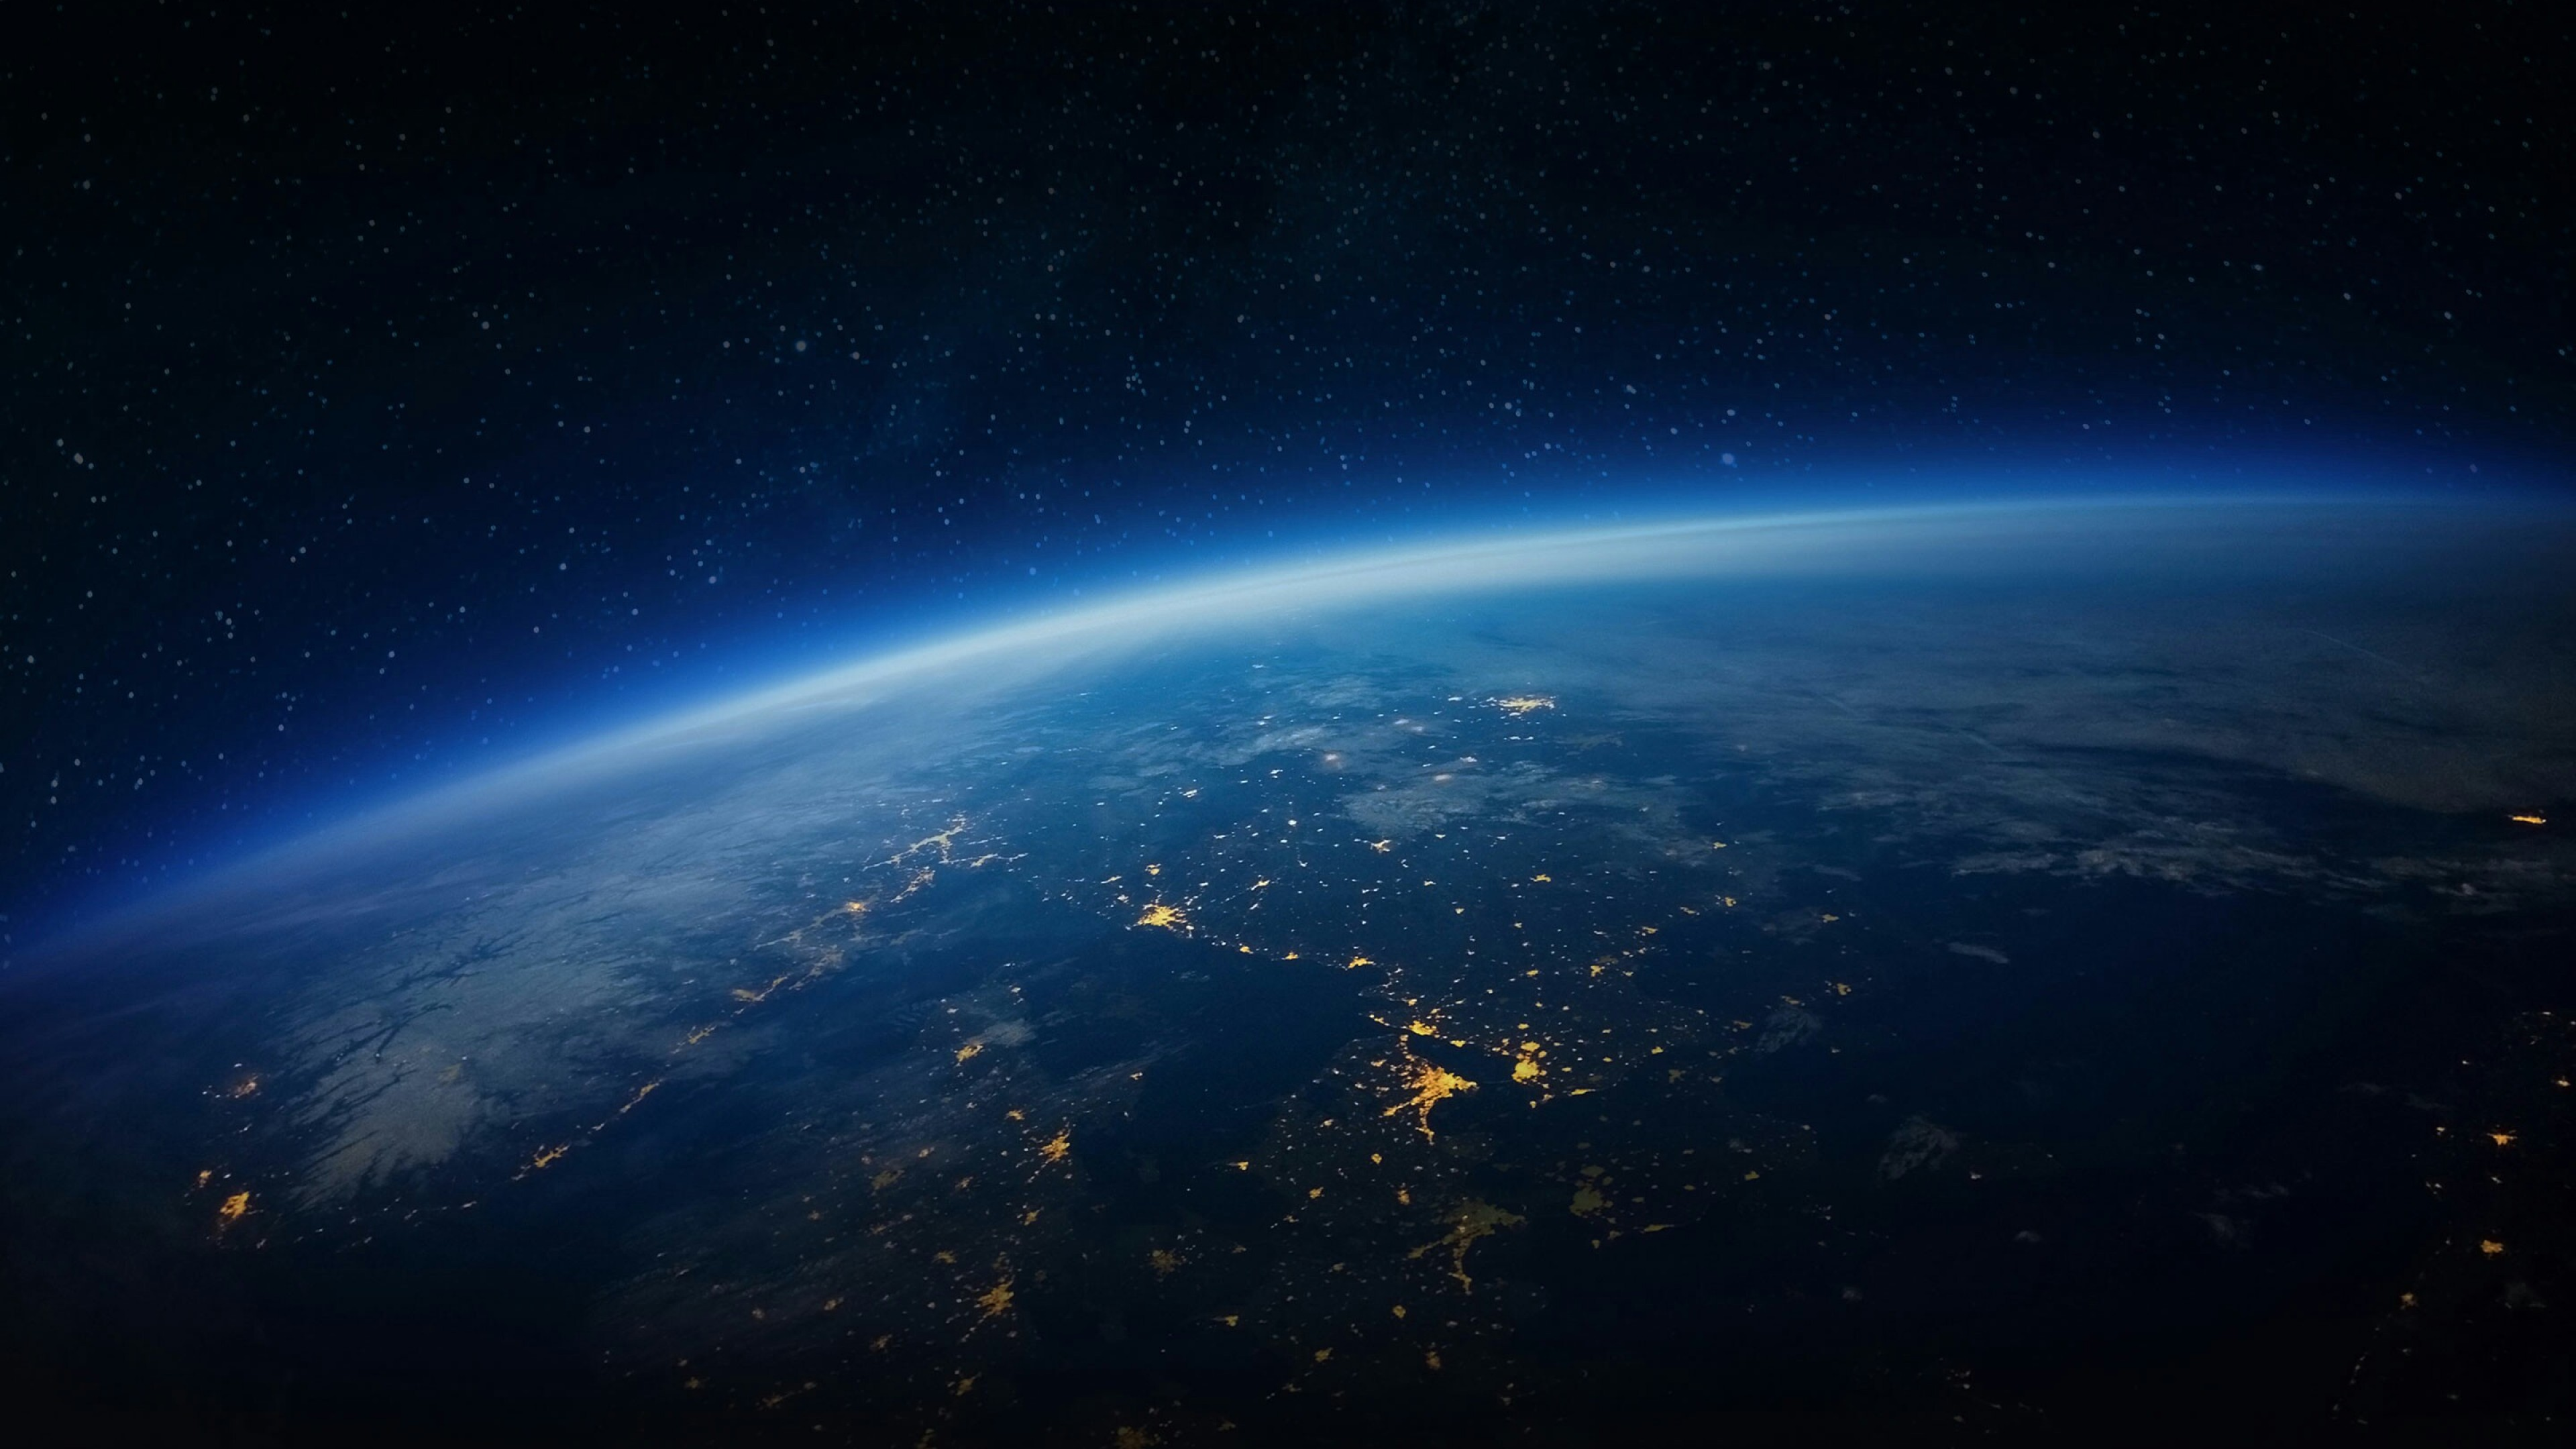
\includegraphics[scale=0.37]{head1}}} 
\centering
\vspace*{5cm}
\par\normalfont\fontsize{35}{35}\sffamily\selectfont
\textbf{{\color{white} Neuronale Netzwerke und Clusteringverfahren für Geodaten}}\\
{\LARGE {\color{white}Lehrstuhl für Geoinformatik}}\par
\vspace*{1cm}
{\Huge {\color{white} Robin Bially}}\par 
\endgroup

%----------------------------------------------------------------------------------------
%	COPYRIGHT PAGE
%----------------------------------------------------------------------------------------

\newpage
~\vfill
\thispagestyle{empty}

%Hier kann ich Github und Downloads hin schreiben
\noindent \textsc{https://github.com/RobinBia/Projektarbeit-Geoinformatik.git}\\ \\ % URL

\noindent Projektarbeit unter der Betreuung von PD Dr. Dr.-Ing. Wilfried Linder von 11.2017 - 09.2018 als Vorbereitung der sich anschließenden Masterarbeit.\\ % 

\noindent \textit{Fertigstellung, August 2018} 


%----------------------------------------------------------------------------------------
%	TABLE OF CONTENTS
%----------------------------------------------------------------------------------------
\raggedright

\chapterimage{head8} % Table of contents heading image

\pagestyle{empty} % No headers

\tableofcontents % Print the table of contents itself

%\cleardoublepage % Forces the first chapter to start on an odd page so it's on the right

\pagestyle{fancy} % Print headers again


%----------------------------------------------------------------------------------------
%	CHAPTER 1
%----------------------------------------------------------------------------------------

\chapterimage{head8} % Chapter heading image

\chapter{Motivation}
\section{leeres Kapitel}
blabla
\chapter{Geodaten und Geoinformation}
\section{Definition und Gestalt von Geodaten}
Geodaten sind digitale Informationen, welche Sachdaten mit Geometriedaten\footnote{https://www.hdm-stuttgart.de/~riekert/lehre gis.pdf} (und Chronometriedaten) vereinen , z.B. \{Luftdruck 1 bar, Ort Düsseldorf, Datum 26.11.2017\}. 
Die räumliche Information kann in unterschiedlichen Formen vorliegen, z.B. symbolisch als Ortsname oder Postleitzahl, aber auch als mathematisch atomare Referenz auf Positionen der Erde mittels Koordinaten. Diese können in unterschiedlichster Dimensionalität vorliegen\footnote{http://www.mathematik.uni-ulm.de/sai/ws04/biosem/GIS.pdf}
\begin{itemize}
\item Ein Objekt ohne bestimmte Länge (0D)
\item Ein Linienstück (1D)
\item
Gauß-Krüger oder geografische Koordinaten mit Bezug auf die Oberfläche der Erde ohne Berücksichtigung von Höhenunterschieden (2D)
\item 
2D-Koordinaten mit einer zusätzlichen Sachinformation für die Höhe über dem Geoiden (2.5D).
\item Kugelkoordinaten mit Bezug auf jeden Punkt im Volumen der Erde als
Geoid oder Rotationsellipsoid (3D)
\item 
Zusätzlich zu den 3 Koordinaten im Raum wird eine vierte
Information mitgeführt, die sich aus dem zeitlichen Ablauf ergibt (4D)
\end{itemize}


\newpage

\section{Geografische Koordinaten}
Ein geeignetes und weit verbreitetes Koordinatensystem zur verzerrungsarmen Darstellung sind die Geografischen Koordinaten. 

\begin{figure}[h]
\centering
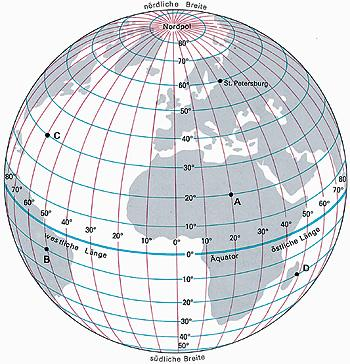
\includegraphics{gradnetz.jpg}
\caption{Das Gradnetz der Erde}\label{gradnetz}
\end{figure}

Beschrieben wird ein Punkt auf der Erde durch gedachte Kreise um den Globus, welche Senkrecht zueinander stehen. Insgesamt existieren 180 Breitenkreise (Richtung Ost-West) und 360 Längenkreise (Richtung Nord-Süd). Die Abweichung von den beiden Referenzkreisen Äquator und Nullmeridian wird in Grad östlicher/westlicher Länge und nördlicher/südlicher Breite angegeben. Als Äquator ($0^\circ$ nördliche/südliche Breite) wird der Breitenkreis bezeichnet, auf welchem die Erdachse senkrecht steht. Der Nullmeridian ($0^\circ$ westliche/östliche Länge) ist der Längenkreis, welcher durch die britische Stadt Greenwich verläuft.\newline Weitere wichtige Koordinatensysteme sind die Gauß-Krüger und UTM-Koordinaten. Die Vorteile dieser Systeme ist, dass sich eine geografische Position direkt ablesen lässt. Geografische Koordinaten erschweren dies bedingt durch die sich verändernden Abstände zwischen den Längenkreisen in zunehmender Nord- oder Südrichtung.


\section{Qualitätsmerkmale}
Ein wichtiger Forschungszweig ist die automatische Beurteilung von Qualitätsmerkmalen von Geodaten hinsichtlich einer bestimmten Fragestellung.
Ein geeignetes Maß ist die gewichtete Summe verschiedener Datenmerkmale, welche in der aktuellen ISO-Norm \textit{ISO 19157:2013}\footnote{https://www.iso.org/standard/32575.html} spezifiziert sind. Die folgende Auflistung ist eine informelle Beschreibung der oben genannten Norm durch Fragestellungen und Beispiele:


\begin{itemize}
\item \textbf{Vollständigkeit}
\begin{itemize}
\item \textbf{Datenüberschuss} -
Enthält der Datensatz mehr Objekte und Beziehungen als angegeben?
\item \textbf{Datenmangel} - Enthält der Datensatz weniger Objekte und Beziehungen als angegeben?
\end{itemize}
\item \textbf{Logische Konsistenz}
\begin{itemize}
\item \textbf{Konzeptuelle Konsistenz} - 
Wurde die Gestalt des Datenmodells bei Aktualisierungen nicht verändert?
\item \textbf{Wertekonsistenz} - Sind alle Werte sinnvoll?
\item \textbf{Formatkonsistenz} Passen die Daten zu angegebenen physikalischen Einheiten?
\item \textbf{Topologische Konsistenz} 
Bleiben topologische Beziehungen bei Änderungen des Datensatzes bestehen (Der botanische Garten befindet sich im Umkreis von 1km von der HHU)?
\item \textbf{Geometrische Konsistenz} - Ist der digitalisierte Datensatz geometrisch sinnvoll und widerspruchsfrei?
\end{itemize}
\item \textbf{Positionsgenauigkeit}
\begin{itemize}
\item
\textbf{Äußere Genauigkeit} - Wie gut stimmen die Koordinatenwerte des Datensatzes mit den wahren Koordinaten überein?
\item \textbf{Innere Genauigkeit} - Wie gut stimmen die relativen Positionen von Objekten zueinander mit den wahren relativen Positionen überein?
\item \textbf{Rasterdatengenauigkeit} - Wie gut stimmen die Rasterdatenpositionswerte mit den wahren Werten überein?
\end{itemize}
\item \textbf{Zeitliche Genauigkeit}
\begin{itemize}
\item
\textbf{Genauigkeit von Zeitmessungen} - 
Wie genau ist die Zeitangabe (minutengenau, taggenau)?
\item \textbf{Zeitliche Konsistenz} - Ist die Reihenfolge der Ereignisse korrekt?
\item
\textbf{Zeitliche Gültigkeit} - Ist der Datensatz in Bezug auf das geforderte Zeitformat korrekt?
\end{itemize}
\item \textbf{Thematische Genauigkeit}
\begin{itemize}
\item
\textbf{Richtigkeit der Klassifikation} - Stimmen Objekte, oder ihre Attribute mit den zugewiesenen Klassen überein, z. B. Zuordnung zu Fluss, statt zu Weg
\item \textbf{Richtigkeit nichtquantitativer Attribute} - Beispiel: Ist das Grundstück wirklich eine Bananenplantage?
\item \textbf{Genauigkeit quantitativer Attribute} - Beispiel: Ist die Fläche des Grundstücks korrekt?
\end{itemize}
\end{itemize}

Viele der oben genannten Punkte lassen einen subjektiven Spielraum für die Bewertung zu. Sowohl Skalierungen als auch Gewichtungen sind nicht eindeutig definiert, was einen Vergleich verschiedener Datensätze erschwert. Aus diesem Grund ist eine algorithmische Interpretation in Kombination mit verfahren der künstlichen Intelligenz hilfreich. So ließe sich aus der Norm ein universeller und allgemeingültiger Indikator zur Bewertung der Datenqualität ermitteln.


\section{Georeferenzierung}
\subsection{Definition}
Unter dem Vorgang der Georeferenzierung,versteht man die Zuweisung raumbezogener Informationen, auch Georeferenz genannt, zu einem Datensatz.

Es gibt folgende vier Arten der Georeferenzierung:

\begin{itemize}
\item Adresskodierung
\item Geotagging 
\item Kartenkalibrierung 
\item Rektifizierung
\end{itemize}

\subsection{Adresskodierung}
Bei der Adresskodierung wird dem Datensatz eine Postanschrift zugewiesen und somit ein indirekter Raumbezug hergestellt. Mithilfe geokodierter Adressen lassen sich funktionale zusammenhänge zwischen Daten, Postanschrift und Adresse herstellen und somit ressourcenschonende und schnelle Zugriffe ermöglichen.
\subsection{Geotagging}
Als Geotagging bezeichnet man das Einfügen eines Attributes (Geotag) inkl. Realweltkoordinate in einen raumbezogenen Datensatz wie ein Bild oder eine Website. Dies ist bei der räumlichen Einordnung der Information hilfreich.
\subsection{Kartenkalibrierung}
Bei der Kartenkalibrierung wird ein räumlicher Datensatz ohne Realkoordinatenbezug mithilfe einer Transformationsvorschrift im Bezug auf die Realwelt so orientiert, dass sich die Koordinaten des Bildes in Realweltkoordinaten einfach umrechnen lassen.
\subsection{Rektifizierung}
Bei der Rektfizierung werden geometrische Verzerrungen in räumlichen Daten entzerrt, indem jedem Datum eine Realweltkoordinate zugeordnet wird.


\subsection{Bestimmung einer Transformationsvorschrift}

Um eine Transformationsgleichung zu finden, werden in der Regel Passpunkte verwendet. Die Passpunkte müssen im Datensatz eindeutig zu erkennen sein. Die Koordinaten der Passpunkte im Realweltkoordinatensystem sind entweder bekannt oder werden einem Referenzdatensatz entnommen. Bei Vektordaten werden die Koordinaten abgegriffen oder interpoliert. Bei Bilddaten werden die Bildkoordinaten der Passpunkte gemessen. Die Transformation sollte unter Berücksichtigung der Abbildungsgeometrie bestimmt werden. Bei Fotos ist somit die Zentralprojektion zu berücksichtigen, bei Karten der entsprechende Kartennetzentwurf. Das automatische Finden von Gemeinsamkeiten in digitalen Bildern und die Bestimmung der Transformation wird in der Bildverarbeitung Bildregistrierung genannt. Die Registrierung von Laserscanning-Punktwolken kann mit dem ICP-Algorithmus erfolgen.\footnote{https://de.wikipedia.org/wiki/Georeferenzierung}

Mark Erweiterungen, implementierungen sinnvoll?

\section{Geoinformationssysteme}
Ein Geoinformationssystem ist eine Software, mit welcher Geodaten erfasst, verwaltet, analysiert und ausgegeben werden können.

Man unterscheidet bei der Abfrage von Daten unter folgenden verschiedenen Typen:
\begin{itemize}
\item Alphanumerische Daten (Attribute als Text oder Zahlen)
\item Text-Dokumente 
\item Multimediale Informationen, wie Videos, Audiosequenzen, Animationen 
\item Fotos, Scans, Satellitenbilder
\end{itemize}

Der Unterschied zu einer Datenbank ist, dass jedes Sachdatum einen expliziten Raumbezug hat, über welchen die Selektion erfolgt. In einer Datenbank erfolgen Zugriffe stattdessen über Schlüsselattribute. Eine weitere Stärke eines GIS ist die grafische Aufbereitung der Daten zur anschaulich-interaktiven Analyse.

Beispiele für solche räumlichen Analysewerkzeuge sind Routenfindung, räumliche Suche. Ein implementiertes Kartografiesystem ermöglicht zudem das markieren von Punkten und Linien, färben von Flächen und die Anzeige und Überlagerung verschiedener Ebenen.

\subsection{Geoobjekte}
Ein Geoobjekt ist ein tatsächlich auf der Erde vorhandenes Objekt, welches durch Geodaten eindeutig referenziert wurde. Man unterscheidet zwischen Gegenständen und Sachverhalten. Gegenstände sind konkrete, visuell wahrnehmbare Erscheinungen auf der Erdoberfläche. Sachverhalte dagegen sind nicht sofort visuell wahrnehmbar, sondern bezeichnen Beziehungen zwischen Gegenständen oder die Interaktion mit der Umwelt und Oberflächengestalt.
Außerdem unterscheidet man zwischen verschiedenen Arten der Datenspeicherung:
\begin{itemize}
\item Flächenhafte Daten
\item Linienhafte Daten
\item Punkthafte Daten
\end{itemize}
Je nach Kartenmaßstab, Auflösungstyp und Speichertyp (digital/analog) werden Daten unterschiedlich repräsentiert. So wird beispielsweise ein flächenhafter quadratischer Gebäudekomplex (10*10 Meter) auf einem Satellitenfoto mit dem Maßstab 1:10.000 nur noch als Punkt wahrgenommen. Linienhafte Daten bieten sich vor allem bei Flüssen, Straßen, Wasser-Land-Grenzen, starken Flankensteigungen usw. an.

\subsection{Modellierung von Geoobjekten}
Die vier informationstechnischen Dimensionen zur Modellierung von geografischen Informationssystemen sind:
\begin{itemize}
\item Geometrie (Ort des Objekts)
\item Topologie (Lage der Objekte relativ zueinander)
\item Semantik (Bedeutung des Objekts im fachspezifischen Kontext, z.B. gut-schlecht, viel-wenig, groß-klein)
\item Dynamik (Änderung des Objekts im zeitlichen Verlauf)
\end{itemize}
Jedes unikate Objekt gehört zu einer Objektklasse, in welcher es nach den oben genannten vier Kriterien beschrieben und mit anderen Objekten der Klasse verglichen wird. Jedes der Objekte besitzt einen eindeutigen Schlüssel zur Identifikation. Möglichkeiten zur Klassifizierung und Clustering von Geoobjekten werden in den folgenden Kapiteln vorgestellt.\newline
Der Ort eines Geoobjektes kann auf zwei verschiedene Arten beschrieben werden:
\subsection{Rastermodell}
Eine analoge topografische Karte oder Zeichnung digitalisiert und in quadratische Gitterzellen aufgeteilt, welche alle über die gleiche Semantik verfügen. Diese Semantik wird stellvertretend durch eine Matrix beschrieben, welche für jede Gitterzelle eine numerische Pixelwertinformation enthält.\footnote{https://de.wikipedia.org/wiki/Geoobjekt}
\begin{figure}[h]
\centering
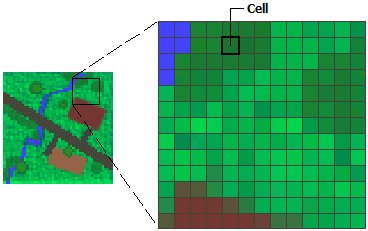
\includegraphics{raster.png}
\caption{Rastermodell-Zoom \protect\footnotemark}
\end{figure}
\footnotetext{http://desktop.arcgis.com/de/arcmap/10.3/manage-data/raster-and-images/what-is-raster-data.htm}

Diese Pixelinformationen repräsentieren Daten wie  Temperatur, Höhe, Vegetationsdichte, Landnutzung, Bodenbeschaffenheit. Rasterdaten werden in der Regel als Bilddatei gespeichert (BMP, GIF, JPEG).
\newline
Die Rastergeometrie eignet sich gut zur Beschreibung flächiger, homogener Sachverhalte. Die einfache Struktur bietet viele Vorteile, aber auch Nachteile: \newline
\textbf{Vorteile}
\begin{itemize}
\item Einfache Datenstruktur 
\item Geeignet für räumliche und statistische Analyse
\item Alles ist einheitlich speicherbar (Punkte, Linien, Polygone)
\item Überlagerung von Ebenen sehr schnell und einfach
\end{itemize}
\textbf{Nachteile}
\begin{itemize}
\item Genauigkeitsverlust beim Scannen und Neustrukturieren
\item Endliche Auflösung => räumliche Ungenauigkeit
\item Pixelwerte haben keine Beziehung zueinander
\item Hoher Speicheraufwand bei Hoher Auflösung, keine Kompression möglich.
\end{itemize}

\subsection{Vektormodell}
Im Gegensatz zu Rasterdaten werden Vektordaten bei linien- und punkthaften Informationen eingesetzt, also Informationen, die sich nicht mit homogener Eigenschaft über die gesamte Karte verteilen. Man nennt solche Informationen auch Features. Beispiele hierfür sind Straßen, Staatsgrenzen, Gewässergrenzen, Höhenlinien, Flüsse, Bäume.
\newline
Eine Punkthafte Vektorinformation wird auch als Vertex bezeichnet. Dieser beschreibt eine Raumlage durch Angabe einer (x,y,z)-Koordinate und ein dazugehöriges Attribut, welches die Art des Punktes beschreibt, z.B. Baum oder Laterne:

\begin{figure}[h]
\centering
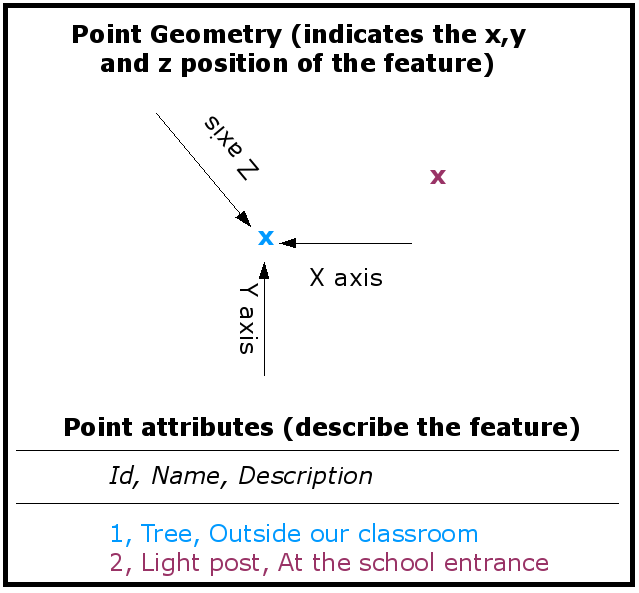
\includegraphics[scale=0.6]{vertex.png}
\caption{Punkt-Feature \protect\footnotemark}
\end{figure}

\footnotetext{https://docs.qgis.org/2.8/de/docs/gentle\_gis\_introduction/vector\_data.html}

Punkteverläufe wie Straßen werden durch sogenannte Polylinien beschrieben. Diese bestehen aus mehreren miteinander verbundenen Vertices. Im Kreis laufende Polylinien bezeichnet man auch als Polygone:

\begin{figure}[h]
\centering
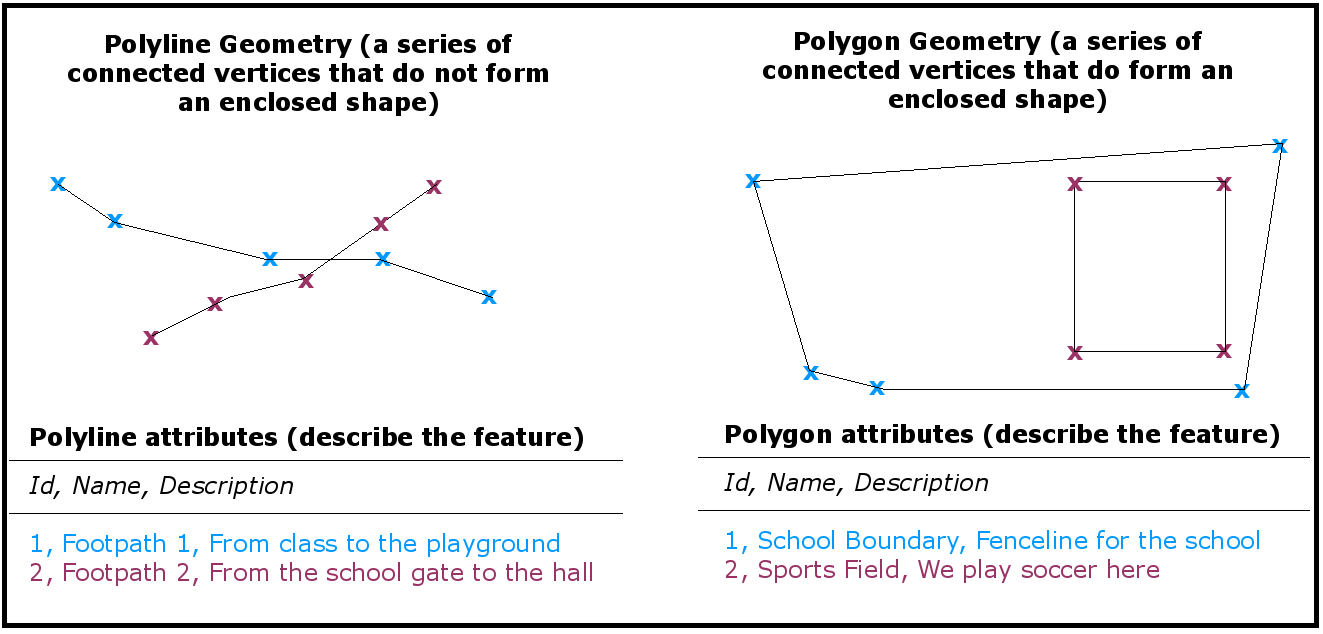
\includegraphics[scale=0.6]{poly.png}
\caption{Polylinien und Polygone \protect\footnotemark}
\end{figure}

\footnotetext{https://docs.qgis.org/2.8/de/docs/gentle\_gis\_introduction/vector\_data.html}

Wie auch bei Rasterdaten gibt es bei Vektordaten nicht nur Vorteile, sondern auch Nachteile.\footnote{http://romanharcke.de/geoinformationssysteme-geodaten-kapitel-4/}\newline
\textbf{Vorteile:}
\begin{itemize}
\item Unendliche Linienauflösung und sehr hohe Genauigkeit
\item Beschreibung von mehreren einzigartigen Features in nur einer Ebene möglich
\item Geringer Speicherbedarf
\item Einfache Erzeugung von Topologie (Knoten, Kanten, Flächen)
\item Gute Performance
\item Ermöglicht Attributierung und Objektdefinitionen
\end{itemize}
\textbf{Nachteile:}
\begin{itemize}
\item Flächenhafte Informationen können nicht gespeichert werden 
\item Durch Scannen können diese Daten nicht erzeugt werden. Es bedarf hier einer Raster-Vektorwandlung (Hoher Erfassungsaufwand)
\item Hoher Rechenaufwand bei Verschneidungen
\end{itemize}

\section{Beispiele von Raster und Vektordaten}
Geodaten müssen heutzutage nicht mehr selbständig erstellt werden. Es gibt eine Vielzahl an staatlichen und privaten Institutionen, welche Ihre Daten kostenlos bereitstellen. So lassen sich zahlreiche Inhalte im ESRI Shapefile Vektordateiformat finden, welches als Quasi-Standard für Desktop-GIS gilt.\footnote{https://de.wikipedia.org/wiki/Shapefile}
Der Datensatz \textit{Natural Earth}\footnote{http://www.naturalearthdata.com/} ist eine Abbildung der Erde im Maßstab 1:10 Millionen. Er ist sowohl als SHP-Vektordatei als auch als Tiff-Rasterbild verfügbar.

Ein ESRI Shapefile besteht aus mindestens drei Dateien zur Speicherung der Geometriedaten, Sachdaten und der Geometrieindizierung zur Verknüpfung von Geometrie und Sachdaten (.shp, .dbf, .shx). Die Geometrie eines Shapefile definiert sich aus nur 4 verschiedenen Formdatenstrukturen: Punkte, Linien, Flächen (Polygone) und Multipunkte.\footnote{http://www.esri.com/library/whitepapers/pdfs/shapefile.pdf}

\begin{figure}[h]
\centering
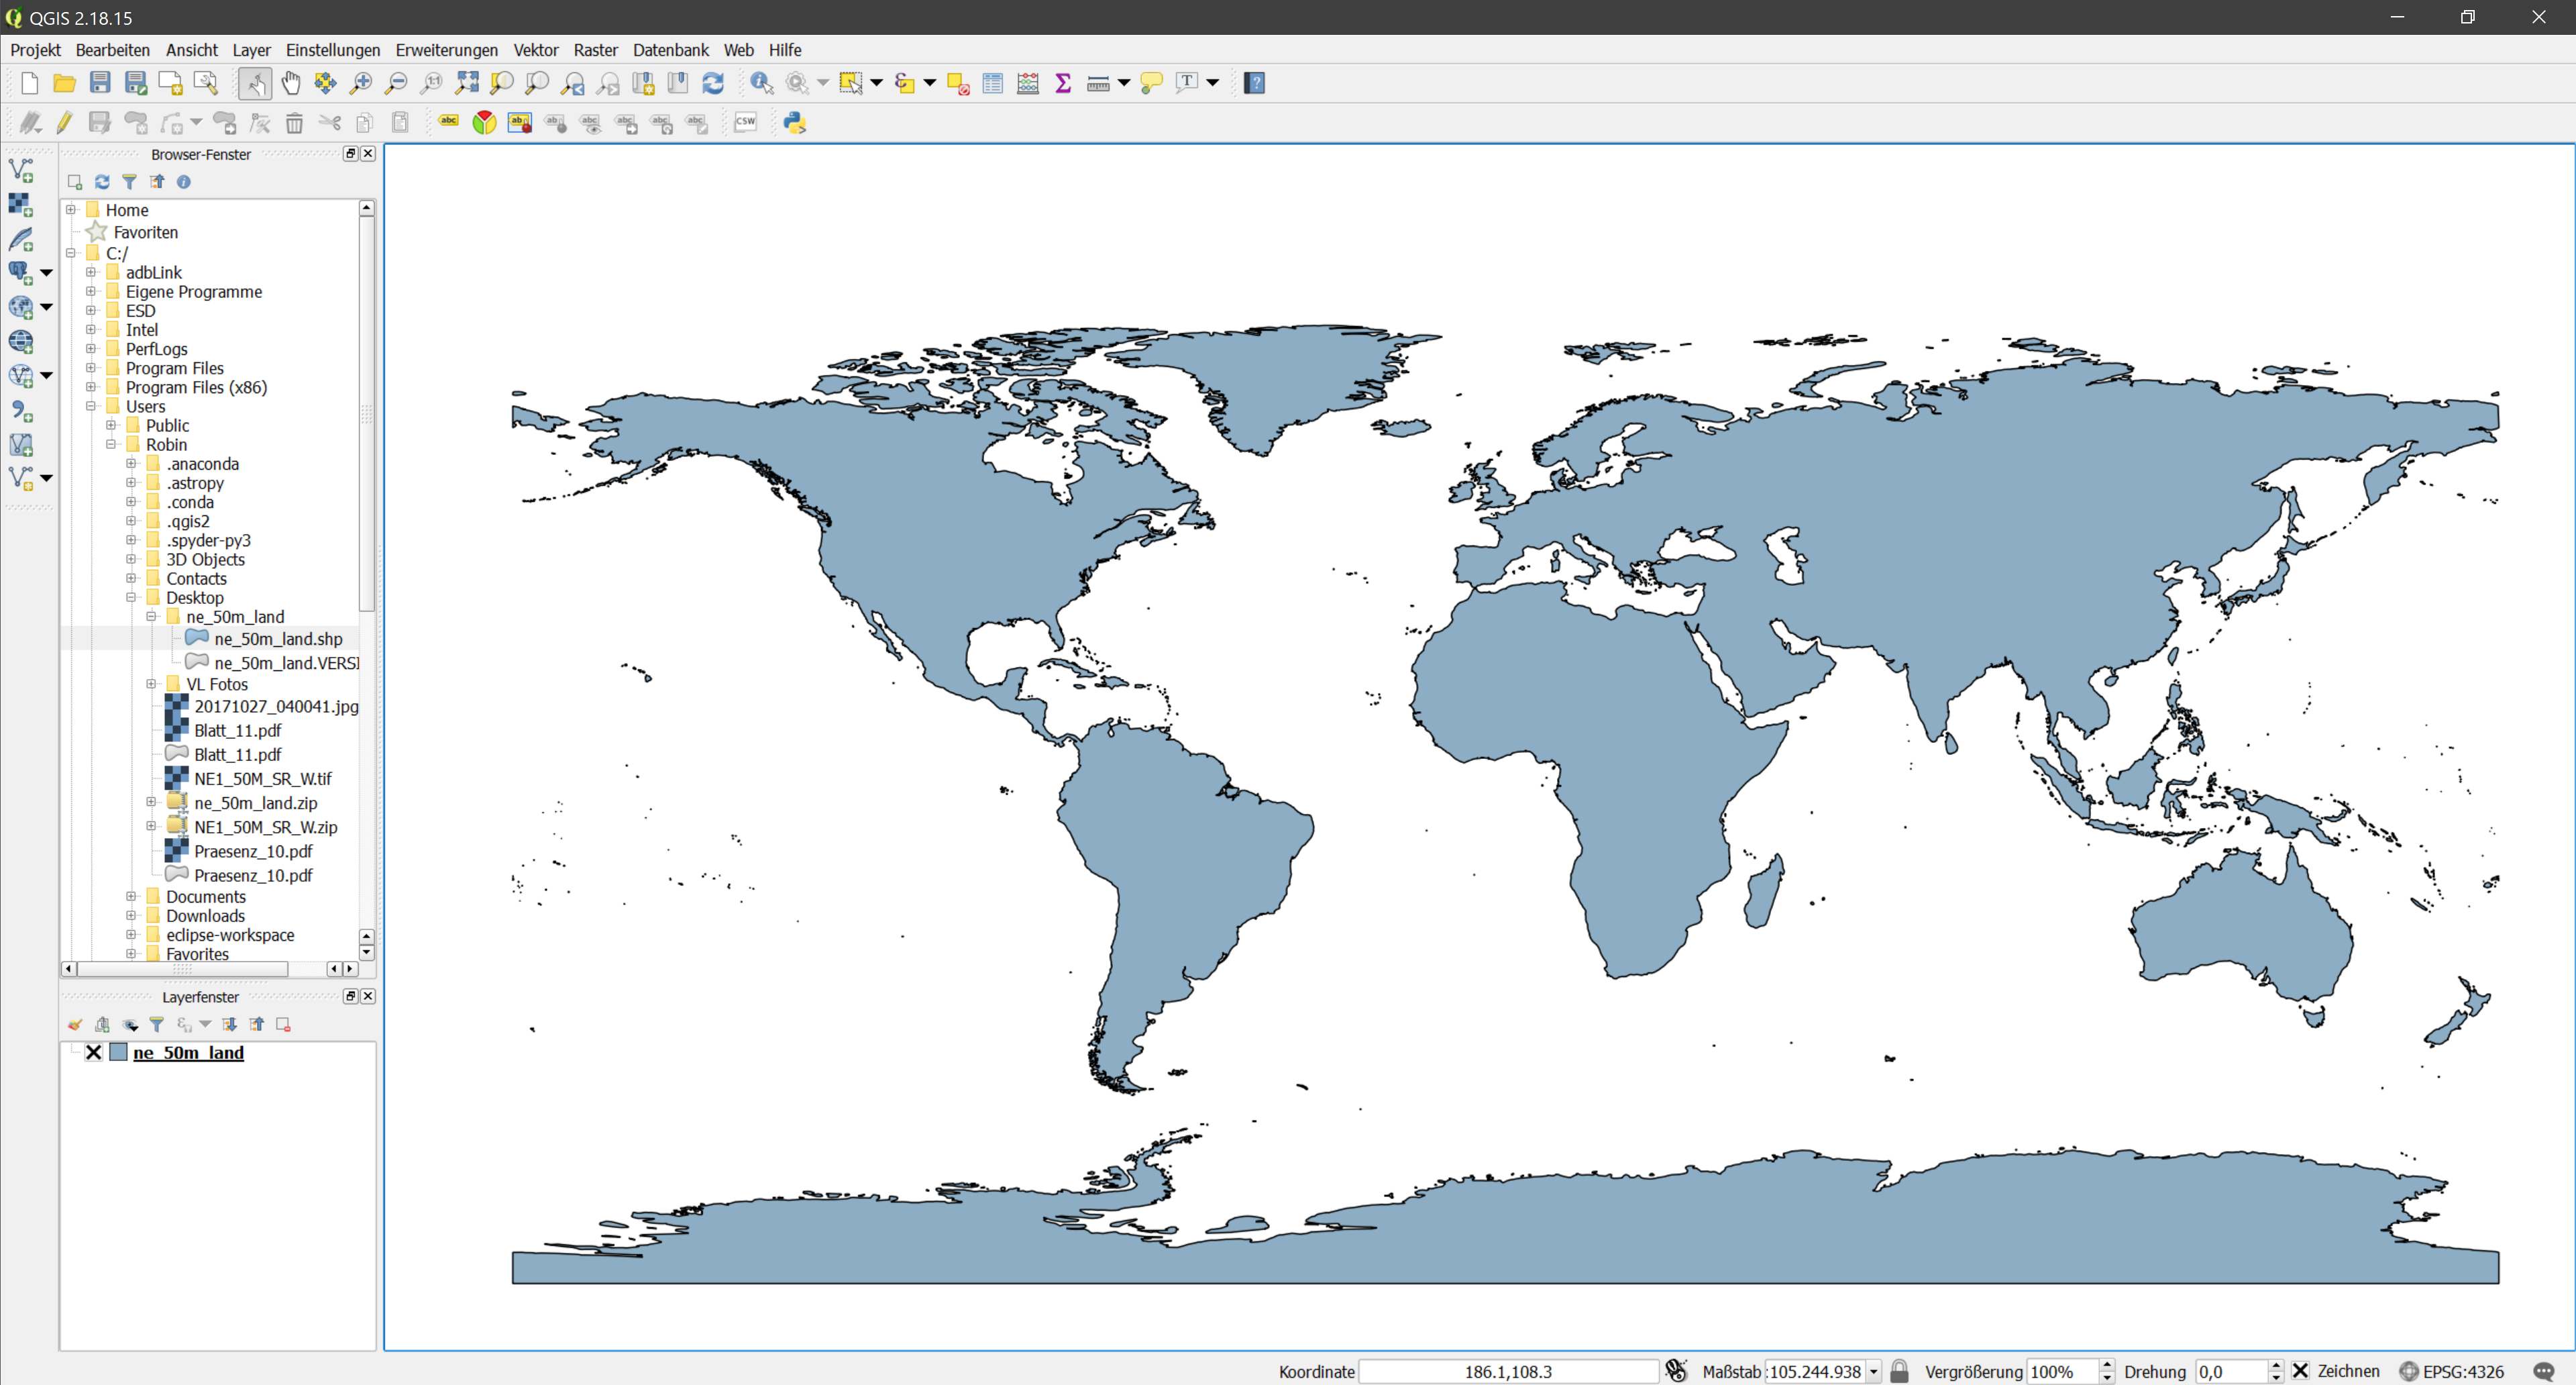
\includegraphics[scale=0.23]{gis.png}
\caption{.shp-Geometriedatei in dem Geoinformationssystem QGIS dargestellt \protect\footnotemark}
\end{figure}
\footnotetext{https://www.qgis.org/de/site/}
Leider eignen sich Vektordaten nicht zur Klassifikation von Features mit Hilfe von Deep Learning wie z.B. Convolutional Neural Networks (CNN), sondern stellen viel mehr das Ergebnis einer Rasterbildanalyse dar. Aus diesem Grund beziehen sich folgende Kapitel im Kontext von Geodaten immer auf Rasterdaten und Bildausschnitte.
\newline
Das dem Datensatz zugehörige farbige Rasterbild inklusive Schummerung (räumliche Schattierung), Wasser und Flüssen sieht so aus:

\begin{figure}[h]
\centering
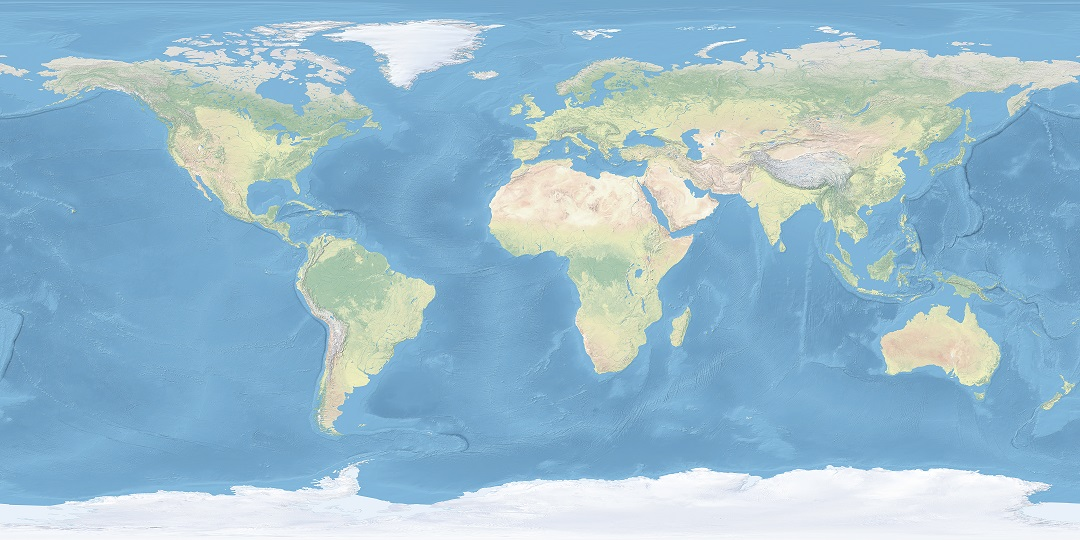
\includegraphics[scale=0.4]{raster_nat_earth.png}
\caption{Rasterbild des Natural-Earth-Datensatzes \protect\footnotemark}
\end{figure}
\footnotetext{http://www.naturalearthdata.com/downloads/10m-raster-data/10m-natural-earth-1/}

\section{Algorithmen in der Geoinformatik}
\section{Verschiedene Arten und ihre Anwendungszwecke}

%----------------------------------------------------------------------------------------
%	CHAPTER 2
%----------------------------------------------------------------------------------------



\chapter{Deep Learning}

\section{Was ist Machine Learning?}
\textbf{Definition}\\
Machine Learning ist eine Unterdisziplin der künstlichen Intelligenz und basiert auf der Idee, biologische Denkprozesse, wie sie in Gehirnen ablaufen, nachzuahmen\cite{geofront}.

\textit{A computer program is said to learn from experience E with
respect to some class of tasks T and performance measure P if its performance at tasks in T, as measured by P, improves with experience E.}\cite{michell}

\bigskip

Ein Computerprogramm lernt also genau dann dazu, wenn es sich hinsitlich seiner Performance in bestimmten Aufgabengebieten mithilfe von Erfahrung selbständig verbessert.

\section{Motivation und Anwendungsgebiete}
Ziel von Machine Learning in den Geowissenschaften ist es, Muster in Geodaten zu erkennen, Vorhersagen zu machen und Phänomene besser erkennen und verstehen zu können.

\bigskip

Eine Stadt ist ein Komplexes System, das aus vielen kleineren interagierenden Subsystemen besteht. Diese werden durch Faktoren wie Politik, Bevölkerungswachstum, Verkehrsinfrastruktur und den Arbeitsmarkt beeinflusst.
Um zu verstehen, welche Kräfte strukturelle Änderungen von Städten vorantreiben, werden sowohl Satellitenbilder als auch nutzerbezogene Positionsdaten aus sozialen Netzwerken wie Facebook und Twitter und Attributierte Markierungen auf Geoinformationssystemen wie OpenStreetMap\footnote{https://www.openstreetmap.org} verwendet, um Langzeitvorhersagen zur erstellen.
Außerdem helfen diese Modelle und Simulationen dabei, die Mechanismen der urbanen Evolution zu erforschen und Städteplanung zu optimieren.

\bigskip

Im Folgenden eine Auflistung verschiedener Probleme, für deren Lösung sich die Anwendung eines Neuronalen Netzwerks eignet:

\begin{itemize}
\item Klassifizierung - Was ist auf einem Bild zu sehen?
\item Lokalisation - Wo ist das Objekt auf dem Bild?
\item Segmentierung - Klassifizierung jedes Pixels
\item Lineare Regression - Lässt sich ein funktionaler Zusammenhang zwischen den Daten des Datensatzes finden, welcher eine Vorhersage zum weiteren Verlauf der Daten ermöglicht?
\item Clustering - Wie lassen sich Daten vergleichen und in Gruppierungen bei gewisser Ähnlichkeit Ihrer Attribute zusammenfassen?
\item Image Captioning - Wie lassen sich die klassifizierten Objekte in Beziehung setzen? 
\end{itemize}

\begin{figure}[h]
\centering
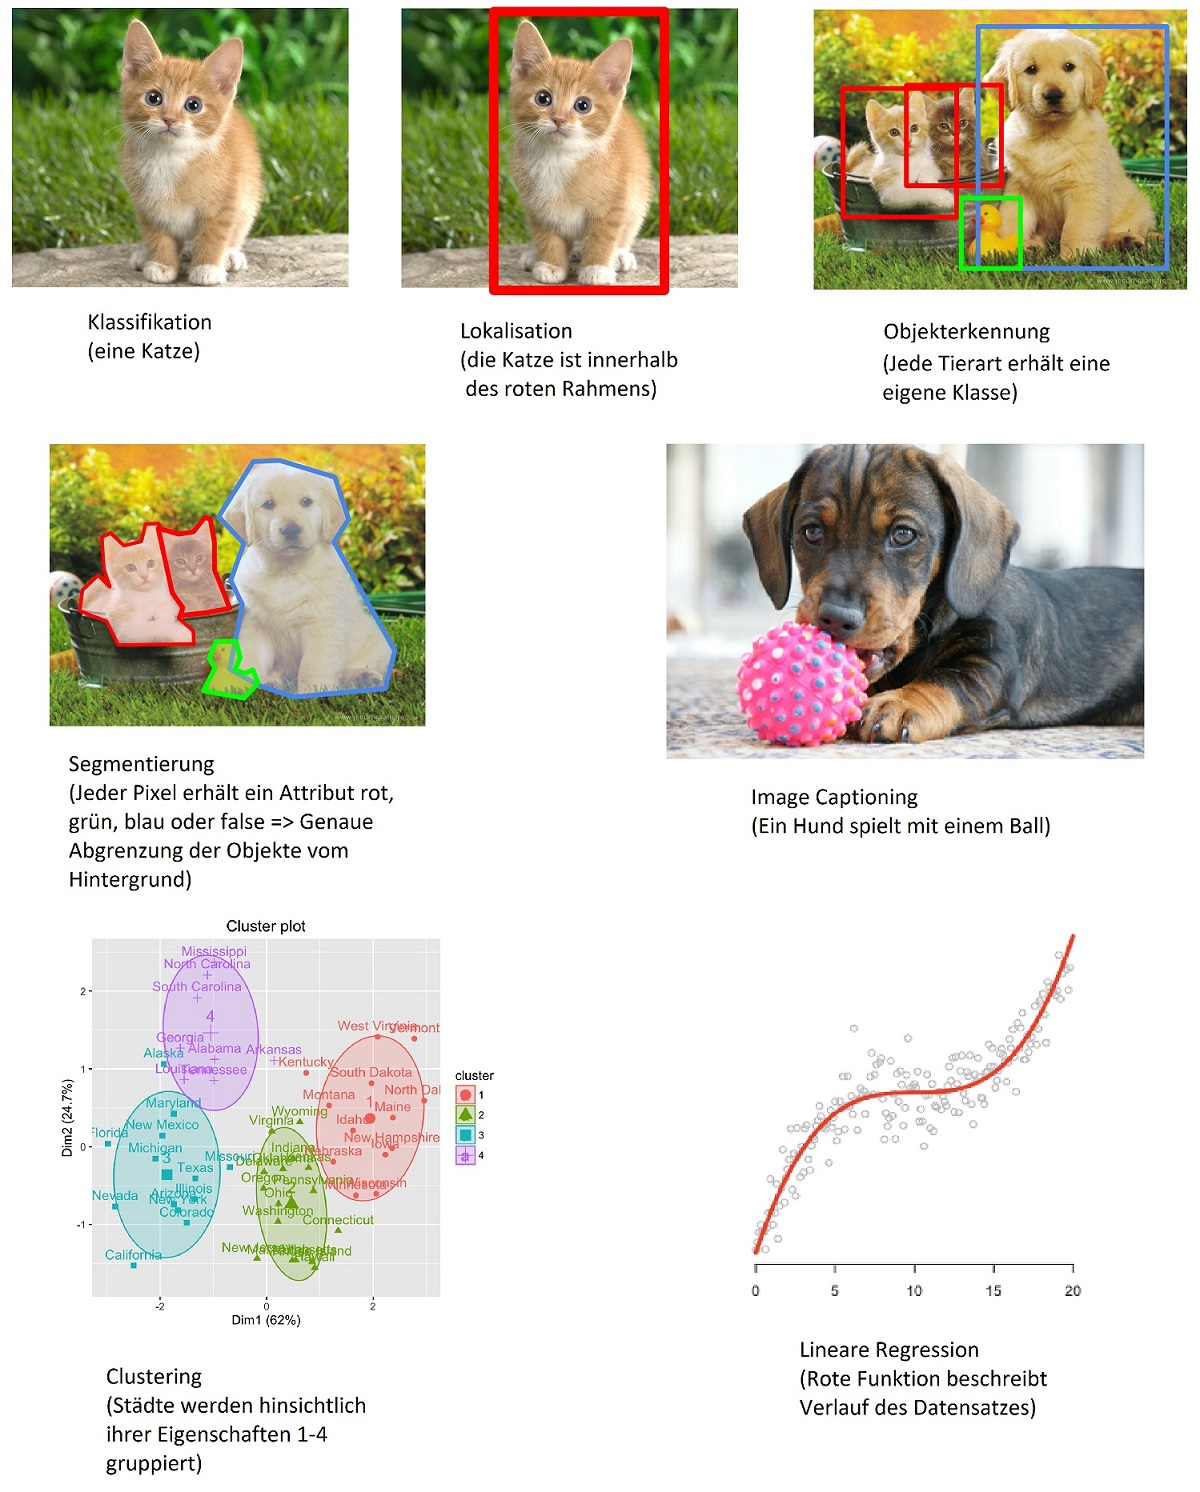
\includegraphics[scale=0.25]{anwendungen.png}
\caption{Vergleich verschiedener Anwendungszwecke von Deep Learning}
\end{figure}

\newpage
\subsection{Linear Classifier}
Um bestimmen zu können, wie gut ein Bild $x$ ($x_i$ sind die einzelnen Pixelwerte) zu einer Klasse $k_j$ passt, muss mithilfe einer Funktion $f$ ein numerischer Vergleichswert bestimmt werden. Die Funktion $f$ wird auch Score-Funktion genannt:

\[f(x_i, W, b) = W \cdot x_i + b \]

Der Parameter $W$ ist die sogenannte Gewichtsmatrix. Sie besitzt die Dimensionalität $i_{max} \times k_{max}$.
Der Parameter $b$ heißt Bias und besitzt die Dimensionalität $k_{max} \times 1$. Er hat die gleiche Funktion wie die Gewichtsmatrix, ermöglicht aber eine zusätzliche additive Änderung beim Lernen. Im nächsten Unterkapitel wird die genauer Erläutert, wie dies zu interpretieren ist.

\begin{figure}[h]
\centering
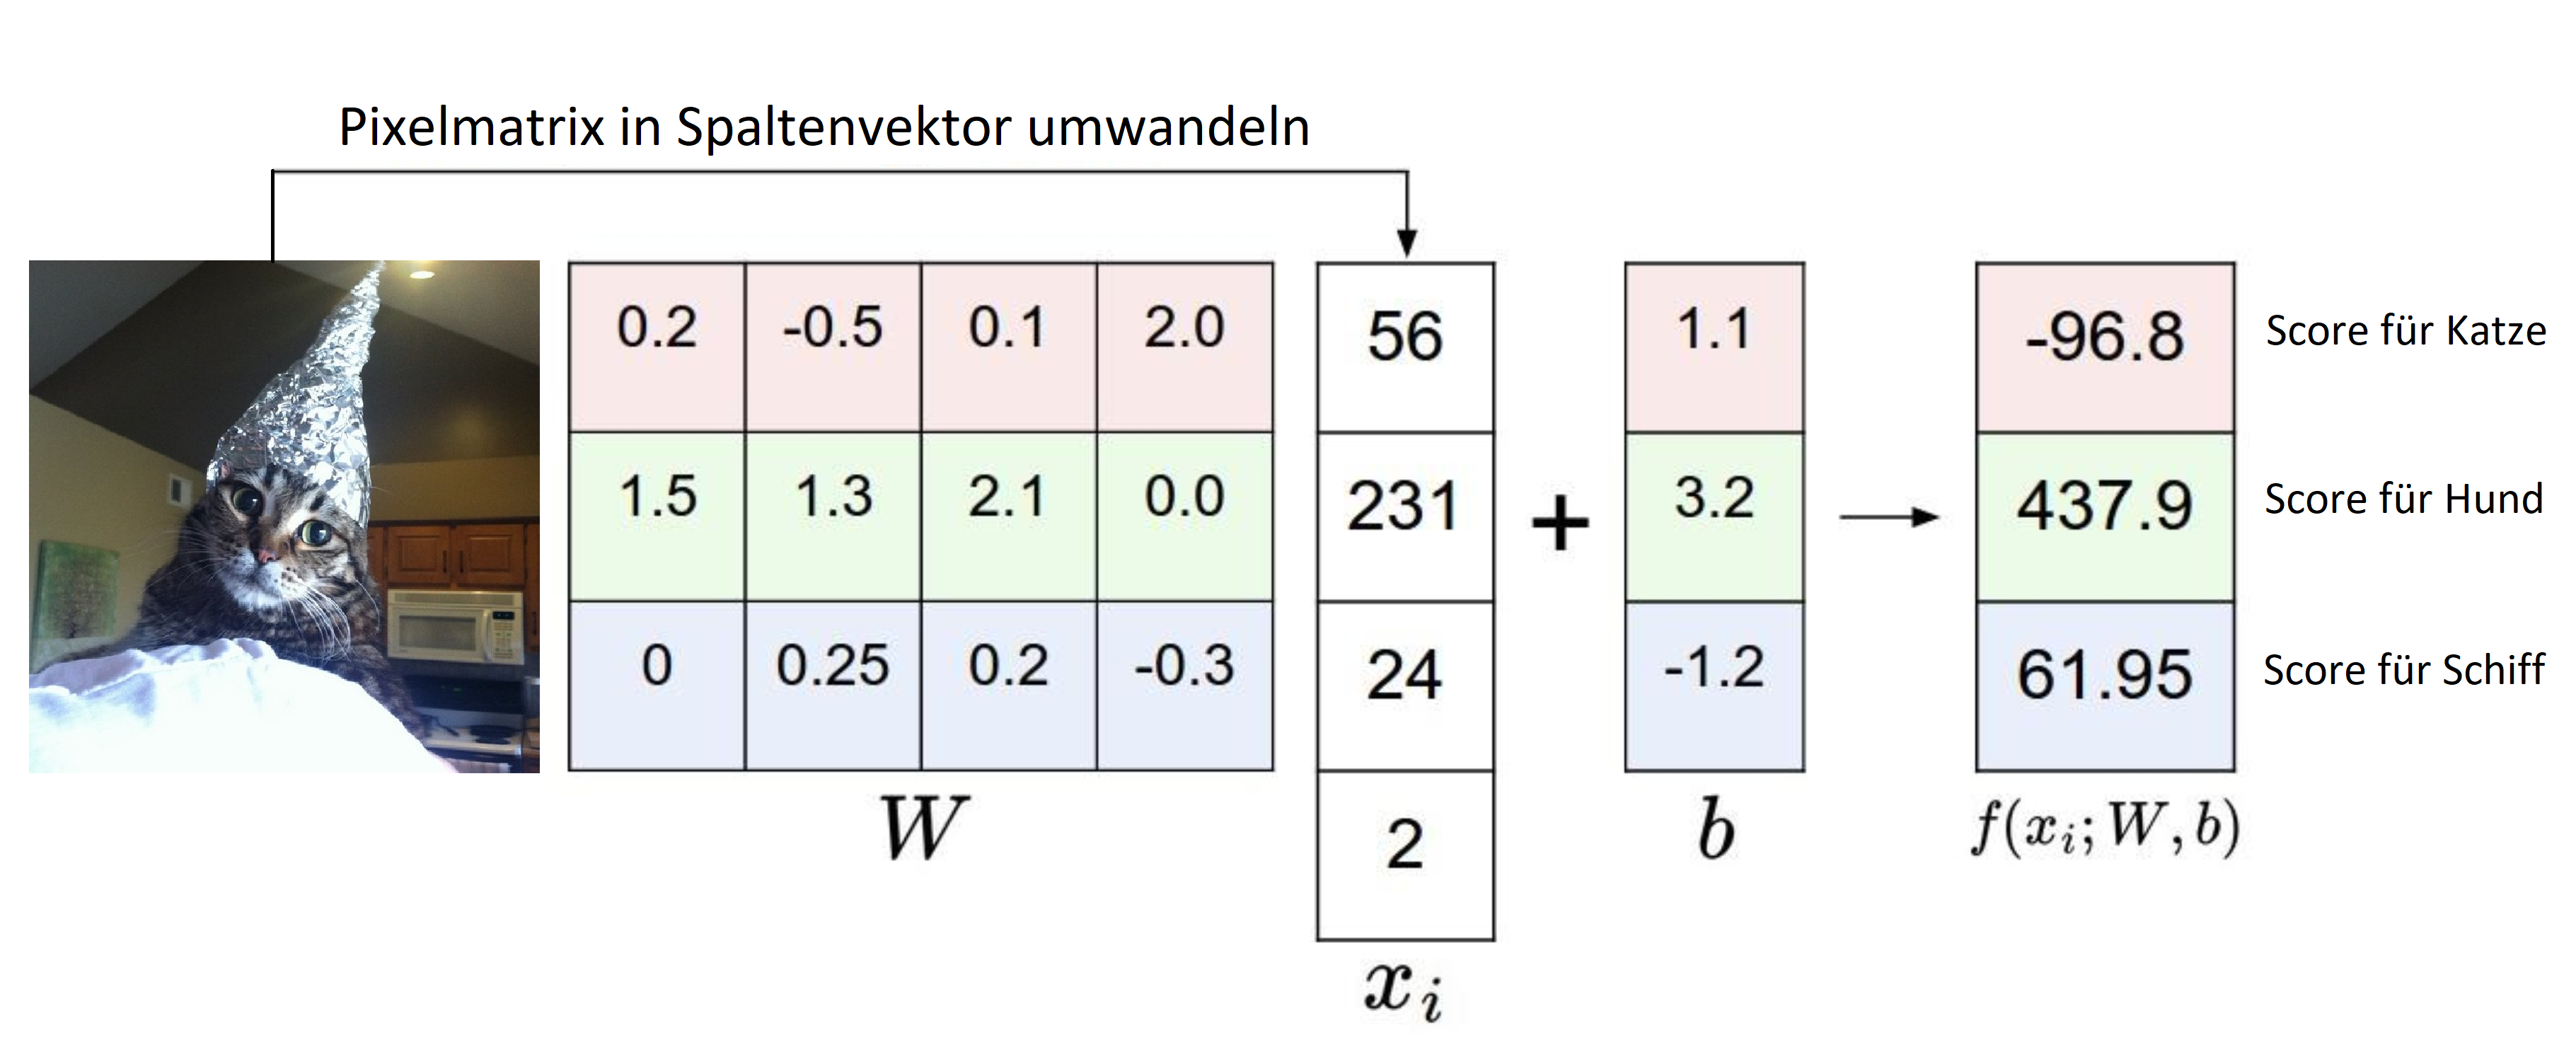
\includegraphics[scale=0.3]{wxplusb.png}
\caption{Interpretation der Score-Funktion anhand eines Beispiels}
\end{figure}

Wenn man ein Bild mit $i_{max}$ Pixeln als $i_{max}$ Dimensionalen Vektor auffasst, dann lässt sich ein Classifier als Hyperebenenseparator dieses Vektorraumes interpretieren. Je höher die Score Funktion für eine Klasse, desto geringer ist der Abstand zum Untervektorraum mit entsprechenden zur Klasse zugehörigen Mustern.

\begin{figure}[h]
\centering
\includegraphics[scale=0.3]{hyperraum.png}
\caption{Hirsch-Auto-Flugzeug-Hyperraum mit Ebenenseparatoren}
\end{figure}

\newpage
Äquivalent zur Score-Funktion definiert man auch eine sogenannte Loss-Funktion. Je besser ein Datum einer bestimmten Klasse zugeordnet werden kann, desto besser sind die Parameter der Gewichtsmatrix und des Bias und desto kleiner der Wert der Loss-Funktion. Im Rahmen eines Optimierungsprozesses soll die Loss-Funktion durch Änderung der Gewichte minimiert werden.
\bigskip
Zwei häufig verwendete Loss-Funktionen für Daten sind:
\begin{itemize}
\item \textbf{Hinge-Loss} $L_i = \sum_{j \neq y_i} max(0,s_j - s_{y_i} + \Delta)$ \Rightarrow Richtige Klasse muss um mindestens Delta größer sein, als alle anderen Klassen
\item \textbf{Softmax-Loss} $L_i = -\log(\frac{e^{s_{y_i}}}{\sum_{j} e^{s_j}})$ \Rightarrow Minimieren der negativen logarithmischen Wahrscheinlichkeit für die korrekte Klasse
\end{itemize}

Der gesamte Loss eines Optimierungsproblems besteht jedoch nicht nur aus dem oben genannten Datenloss, sondern des Weiteren aus dem Regularisierungs-Loss.

\subsection{Regularisierer}
Ein Regularisierer soll verhindern, dass sich die Gewichte immer nur hinsichtlich einer bestimmten Klasse verändern. Zum Beispiel kann es sein, dass ein Netzwerk, das ohne Regularisierer trainiert wurde zwar gut Katzen erkennen kann, jedoch keine Hunde. Das Ziel ist hierbei also, ein Netzwerk zu erzeugen, dass die Generalisierung "Tier" versteht und darüber hinaus zwischen verschiedenen Tierarten unterscheiden kann. Eine Möglichkeit, dies zu realisieren, bieten Bestrafungsterme:

\[R(W) = \sum_{k}\sum_{l} W_{k,l}^2\]

Dieser Bestrafungsterm geht ebenfalls in die Loss-Funktion mit ein. Die Quadrierung der Gewichte sorgt dafür, dass zuvor bereits deutlich größere Gewichte in der Loss-Funktion umso mehr berücksichtigt werden. Im Laufe des künftigen Trainingsprozesses können Ausreißer effektiv erkannt und vermieden werden. Die Loss-Funktion wird nur dann minimal sein, wenn sich die Gewichte nicht zu stark voneinander unterscheiden.
\\
Die gesamte Loss-Funktion lautet also:
\[L_{ges} = \frac{1}{N} \sum_{i} L_i + \lambda R(W)\]

\subsection{Gradientenabstieg}
Um die Loss-Funktion zu minimieren, müssen die Gewichte $W$ aktualisiert werden. Hierzu berechnet man den negativen Gradienten (Partielle Ableitungen der Loss-Funktion nach den Gewichten). Auf der Ebene, welche die Loss-Funktion aufspannt, zeigt der Gradient in Richtung des steilsten Abstiegs.


\subsection{Multi-Layer Neural Network}
Ein Multi-Layer Neuronales Netzwerk ist ein gerichteter azyklischer Graph, wobei die Knoten in Ebenen angeordnet werden. Die erste Knotenebene besteht aus den Eingabedaten. Im Bildbeispiel wäre jeder Knoten ein Pixelwert. Die Kanten des Graphen entsprechen den Werten der Gewichtsmatrix $W$. Die Knoten der Hidden-Layers under der Output-Layer lassen sich als Neuronen interpretieren, welche durch Aktivierung oder Deaktivierung bestimmte Muster der Eingabedaten lernen. Ob ein Neuron aktiviert wird oder nicht, bestimmt die Aktivierungsfunktion $g$. Das Ergebnis wird an eine weitere Neuronenschicht weitergeleitet und die gelernten Muster somit weiter verfeinert.

\begin{figure}[h]
\centering
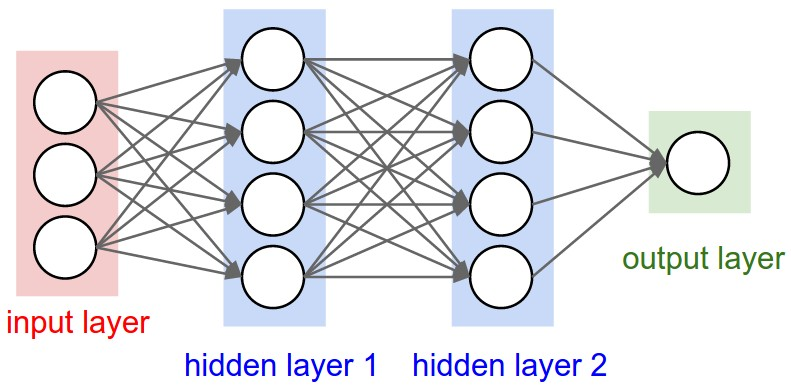
\includegraphics[scale=0.35]{mlnn.png}
\caption{Multi-Layer NN. mit 2 Hidden-Layers, 32 Gewichten, 9 Biases und 9 Neuronen}
\end{figure}

Die Score-Funktion für dieses Netzwerk lautet:

\[y(x) = W_3^T \cdot g[W_2^T \cdot g[W_1^T \cdot x+b_1]+b_2]+b_3\]


\subsection{Trainieren eines Netzwerks mittels Backpropagation}
Sei $f$ eine Score-Funktion für ein Single Layer Neural Network mit nur einer Aktivierung.

\[f(x,w) = \frac{1}{1+e^{-(w_0x_0+w_1x_1+w_2)}}\]

Diese Aktivierungsfunktion nennt sich auch Sigmoidfunktion. Sie transformiert relle Zahlen auf ein Intervall $\left[0, 1\right]$.

\begin{figure}[h]
\centering
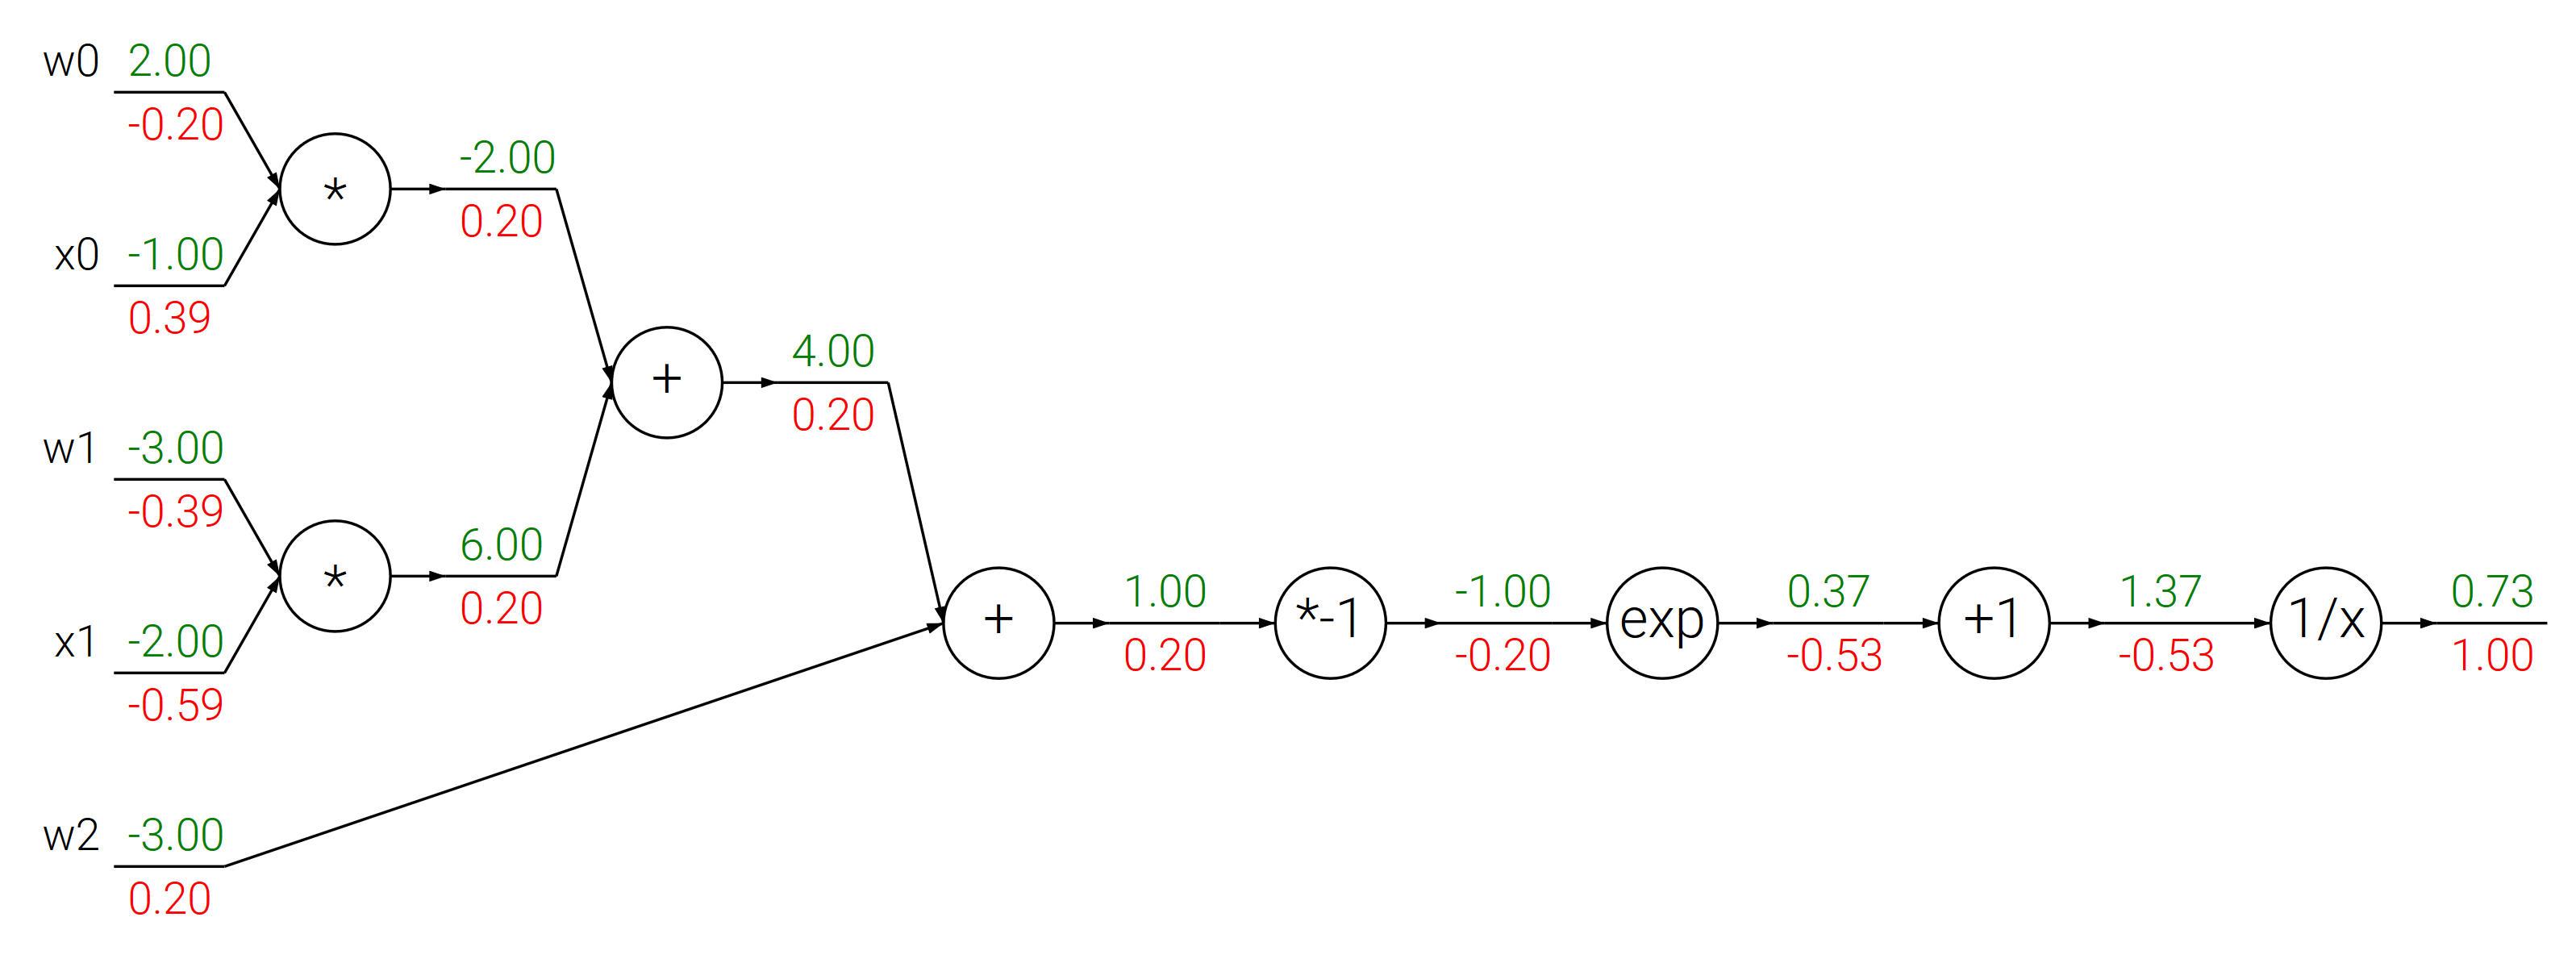
\includegraphics[scale=0.3]{sigmoid.png}
\caption{Beispiel für Backpropagation anhand der Sigmoid-Funktion}
\end{figure}

Das Ergebnis von $f(x,w)$ mit $w = (2,-1,-3)$ und $x = (-1,-2)$ ist $0.73$. Die Ableitung von  $\frac{1}{x}$ ist $-\frac{1}{x^2}$. Anschließend rechnet man $-\frac{1}{1.37^2}\cdot 1 = -0.53$. Die Ableitung von $x+1$ ist $1$. Also rechnet man $1\cdot -0.53=-0.53$. Die Ableitung von $e^x$ ist $e^x$. Man rechnet $e^{-1}\cdot 0.53=-0.2$. Diese Vorgehensweise entspricht der Anwendung der Kettenregel. Fährt man fort, erhält man Gewichtsänderungen $W_{exch}=(-0.2,-0.4,0.2)$. Diese Änderungen subtrahiert man von den alten Gewichten mit einem Parameter $step$: $W \minuseq step \cdot W_{exch}$. Dabei gibt Lernrate $step$ an, wie stark die Änderung der Gewichte ausfallen soll. Eine zu große Änderung kann bedeuten, dass man über das Minimum der Loss-Funktion hinaus springt. Sind die Änderungen zu klein, so muss der Gradient oft berechnet werden, was sehr lange dauern kann. Das Ergebnis der Score-Funktion für $W' = (1.8,-3.4,-2.8)$ ist $0.9$. Das Netzwerk klassifiziert nun also besser.\\
\bigskip
Neben der Sigmoidfunktion gibt es noch viele andere Aktivierungsfunktionen. So hat die Maximumsfunktion (Rectifier Linear Unit - ReLU) gegenüber der Sigmoidfunktion den Vorteil, dass bei relativ hohen Werten nicht alle Neuronen aktiviert werden und es somit weiterhin zu einem Lerneffekt kommt. Ein weiterer Vorteil des Recitifiert ist die schnellere Konvergenz des Gradienten. So stellt sich bereits nach wenigen Trainings ein starker Lerneffekt ein. Sind die gewichte jedoch zu Beginn sehr klein, so ist die Gefahr groß, dass bei einer weiteren Verkleinerung alle Neuronen deaktiviert werden.

\begin{figure}[h]
\centering
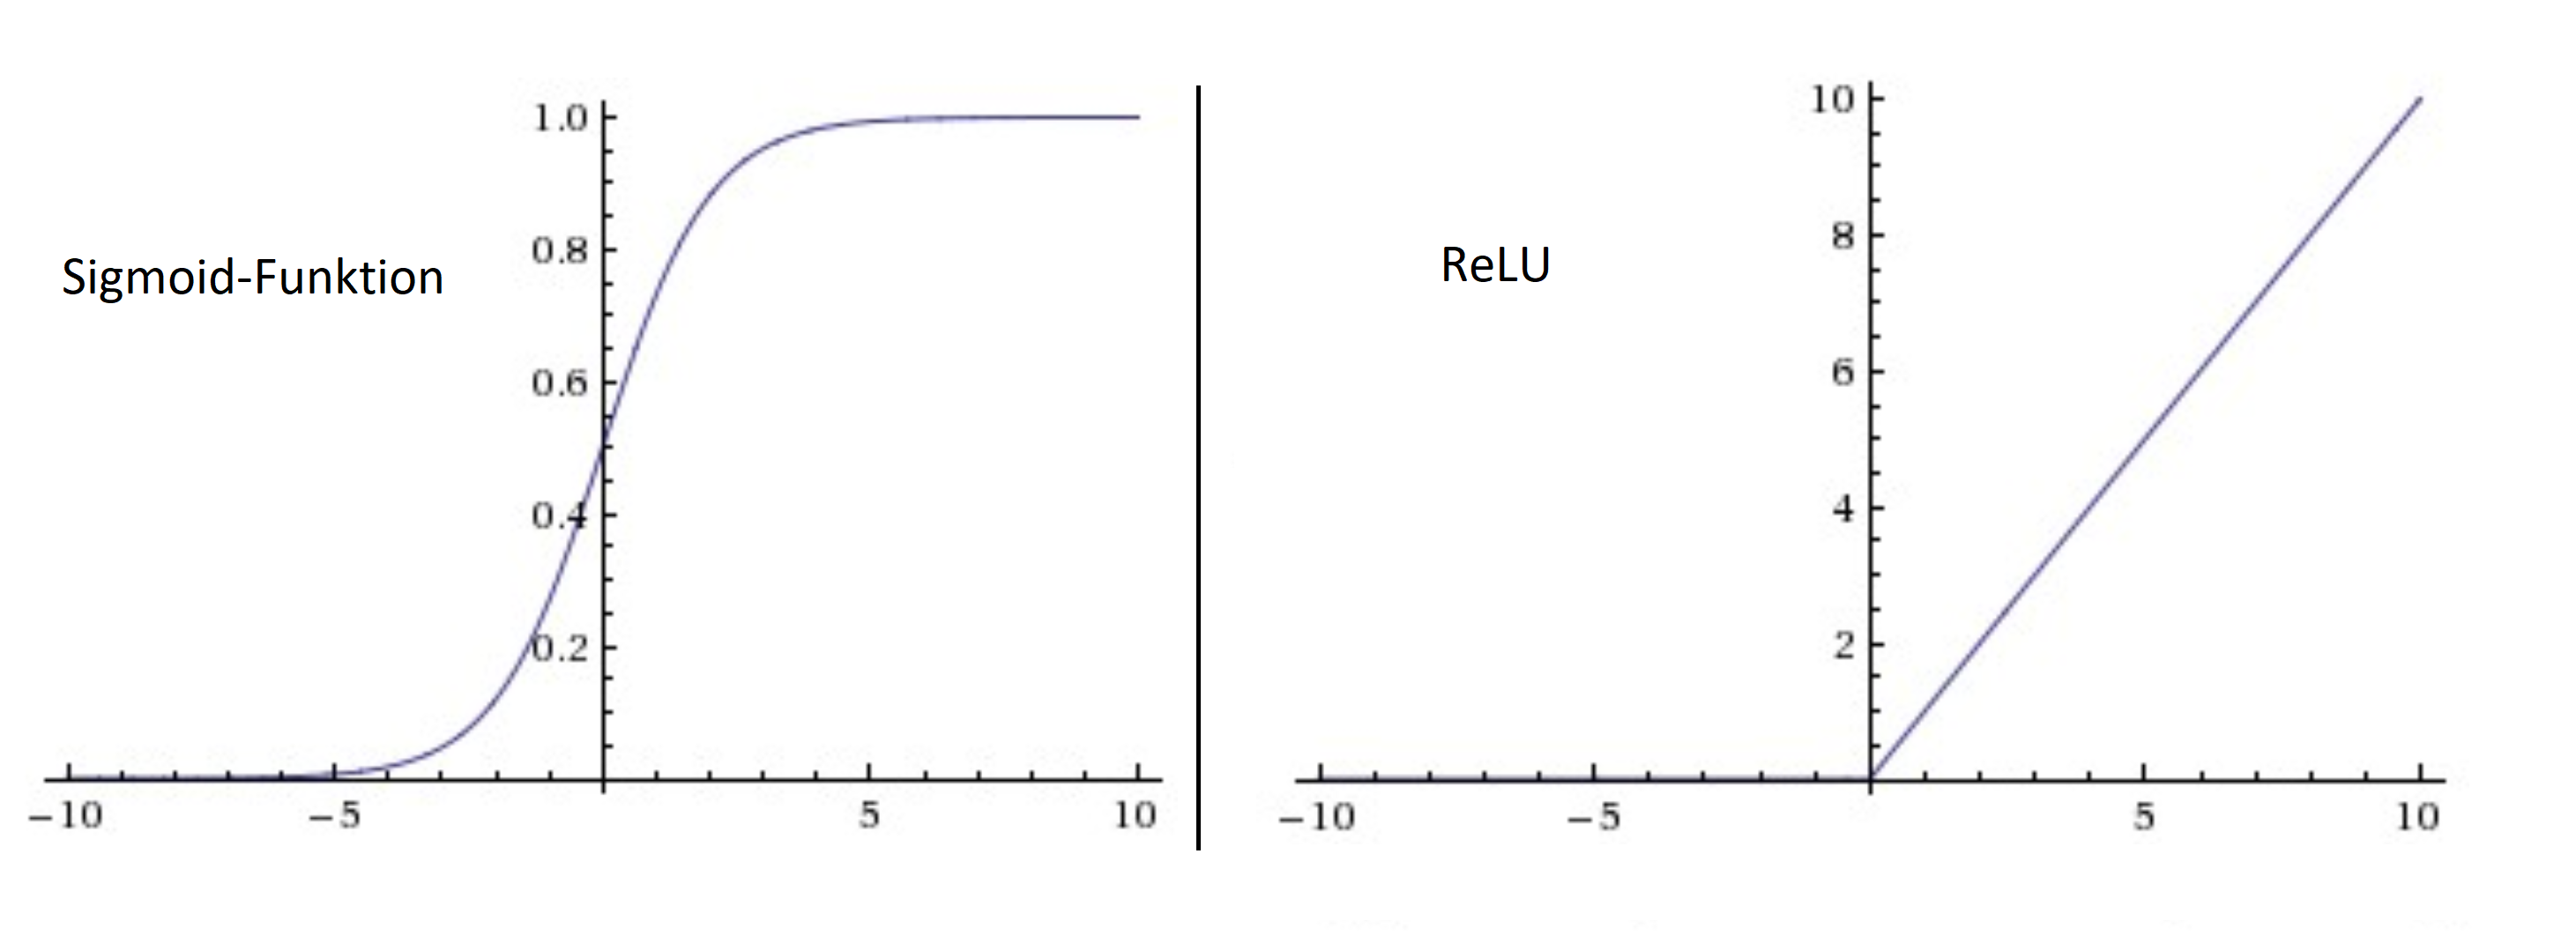
\includegraphics[scale=0.3]{aktf.png}
\caption{Vergleich zwischen Rectifier und Sigmoid}
\end{figure}

\subsection{Parameterupdates\protect\footnote{http://ruder.io/optimizing-gradient-descent/}}
\textbf{Batch Gradient Descent (BGD)}
Normaler einmaliger Updateprozess wie oben beschrieben. Diese Variante ist sehr langsam, da für jedes Update der Gradient für den gesamten Datensatz berechnet werden muss.
\[W = W - \eta \nabla_WL(W)\]

\textbf{Stochastic Gradient Descent (SGD)}
In diesem Fall werden die Gewichte nach jedem Trainingsbeispiel aktualisiert. Dies beschleunigt den Trainingsprozess und verhindert Redundanzen:

\[W=W - \eta \nabla_W L(W;x_i)\]

\bigskip
Zur Beschleunigung des Gradientenabstiegs wurden ebenfalls Verfahren entwickelt:
\begin{itemize}
\item \textbf{Momentum} Falls der Gradient zu groß ist, wird das Ziel beim aktualisieren der Gewichte übersprungen. Diese Methode beschleungigt den Gradientenabstieg, indem die Anzahl der übersprungenen Minima reduziert wird (quantitative Oszillationsreduktion). Hierzu wird der Update-Vektor des vorherigen Schrittes durch einen Paramter $\gamma$ gewichtet und zum neuen Update-Vektor addiert:

\[v_t=\gamma v_{t-1}+\eta \nabla_WL(W)\]
\[W=W-v_t\]

\begin{figure}[h]
\centering
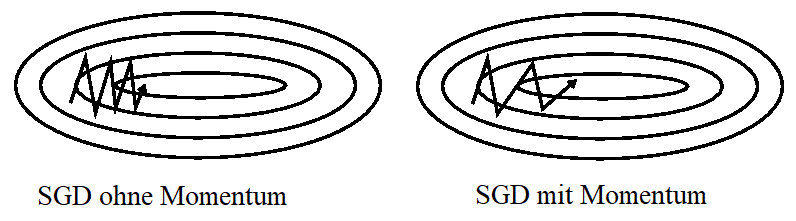
\includegraphics[scale=0.7]{momentum.png}
\caption{Momentum verringert die Oszillation der Loss-Funktion}
\end{figure}



\item \textbf{Adagrad} Dieses Verfahren findet für jeden Parameter in jedem Updateschritt eine individuelle Lernrate. Dies bewirkt, dass das Minimum bei starker Steigung nicht übersprungen wird. Die Oszillation wird qualitativ reduziert.

\[W_{t+1,i}= W_{t,i} - \frac{\eta}{\sqrt{G_{t,ii}+\epsilon}} \nabla_W L(W_{t,i})\]

Wobei $G_{t}$ eine Diagonalmatrix ist und das Element $i,i$ ist die Summe der Quadrate der Gradienten bezüglich $W_t$ bis Zeitschritt $t$. Das $\epsilon$ verhindert eine Nulldivision.
\end{itemize}

\subsection{Convolutional Neural Network}
Ein Convnet ist ein Neuronales Netzwerk, das speziell für das Klassifizierungproblem geeignet ist. Ein Standardnetzwerk besteht aus folgenden vier Layern:

\begin{itemize}
\item \textbf{1. Convolution Layer} Dies ist ein Filter $W$, der Dimension $F \times F\times c$, wobei das Bild $P$ die Dimension $N\times N\times c$ hat und $N>F$. Die neue Größe (Höhe/Breite $N$) des Ausgabebildes nach der Convolution beträgt $\frac{N-F}{stride+1}$, wobei der Stride die Anzahl der Gitterzellen ist, die der Filter jedes mal weiter springt. Als Padding bezeichnet man die Anzahl der Gitterreihen, die um das Ursprungsbild herum virtuell angefügt werden, um zu verhindern, dass das Bild durch die Convolution kleiner wird. Zu Beginn wird der Filter an die linke obere Ecke angesetzt. Anschließend wird der erste Wert des neuen Bildes berechnet.

\[\sum_{i=1}^F \sum_{k=1}^F{P_{i,k} \cdot w_{i,k}}\]

Danach wird der Filter um $stride$ Gitterzellen nach rechts verschoben und es wird erneut aufsummiert.

\begin{figure}[h]
\centering
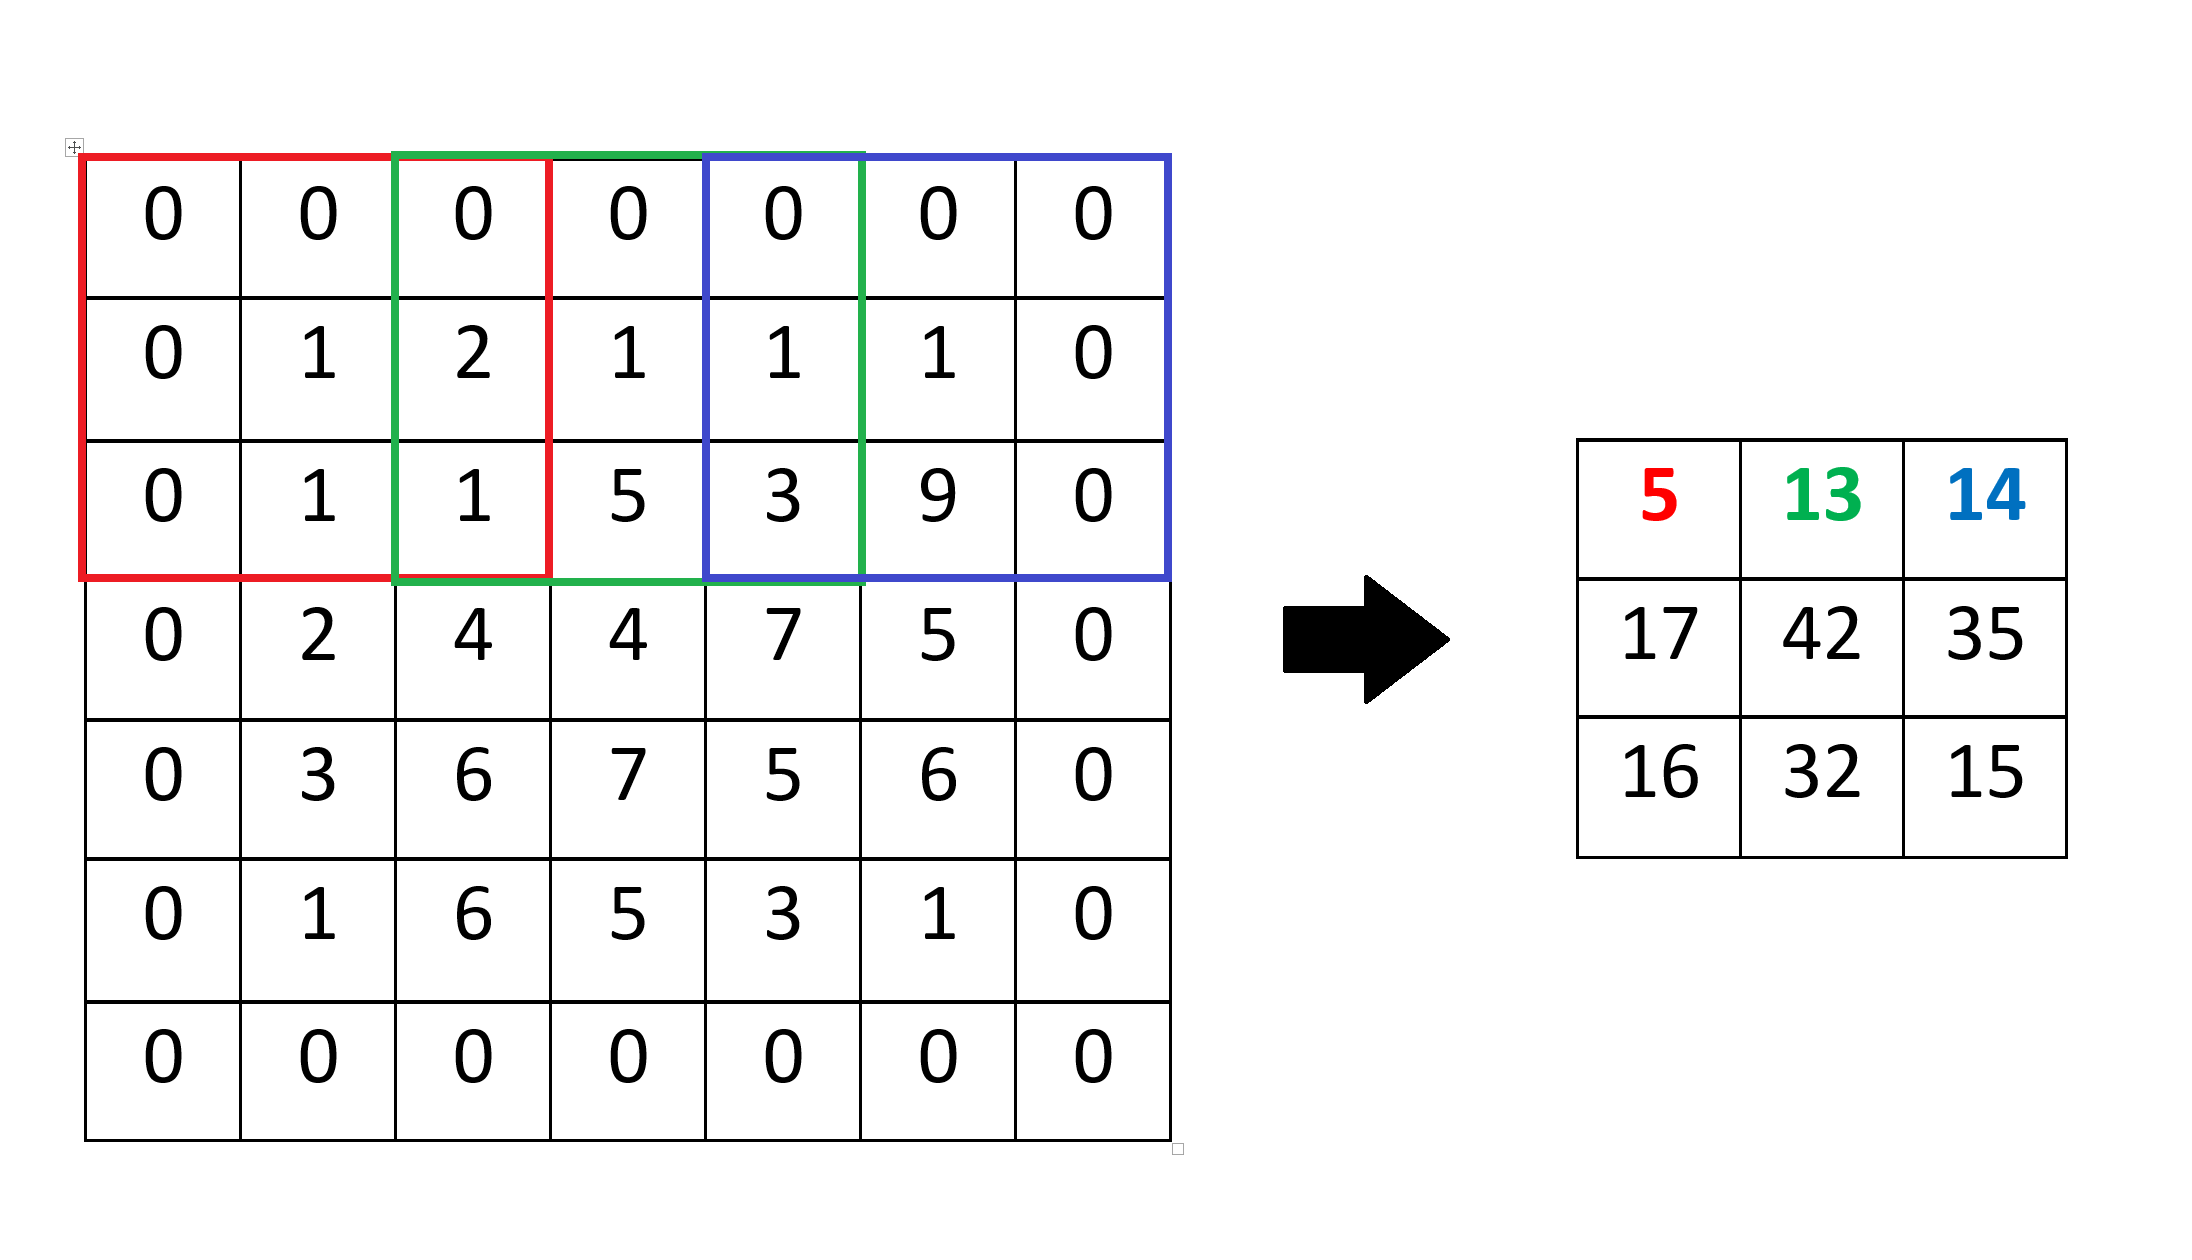
\includegraphics[scale=0.3]{convolution.png}
\caption{Convolution eines $7 \times 7$ Bildes mittels $3 \times 3$ Eins-Filter ($w_{i,k} = 1$), Padding = 1 und Stride = 2}
\end{figure}

Jeder Filter erstreckt sich über die gesamte Tiefe des Bildes. Wird also ein $B\times B\times 3$ Filter auf ein $A\times A\times 3$ Bild angewandt, so hat das Ausgabebild die Dimension $C\times C\times 1$ mit $C = \frac{A-B}{stride+1}$. Werden $10$ Filter der größe $B\times B\times 3$ angewandt, so hat die Ausgabe die Dimension $C\times C\times 10$. Je mehr Filter angewandt werden, desto besser können Muster gelernt werden. Zu große und zu kleine Filter führen zu Over- und zu Underfitting.

\item \textbf{2. ReLU Layer} Diese Layer übernimmt das Aktivieren der einzelnen Gewichte mit z.B. max(0,x).

\item \textbf{3. Pooling Layer} Diese Layer reduziert die Ausgabe nach der Filterung und Aktivierung auf wesentliche Merkmale des Bildes und verkleinert die Anzahl der Pixel, die für die Speicherung dieser Merkmale notwendig sind. Zum Einsatz kommt meistens das Max-Pooling. Hierbei wird wie bei der Convolution eine Maske auf das Bild gesetzt. Das Maximum aller Bildwerte, die sich hinter der Maske befinden, ist der Wert des neuen Bildes nach dem Pooling. 

\begin{figure}[h]
\centering
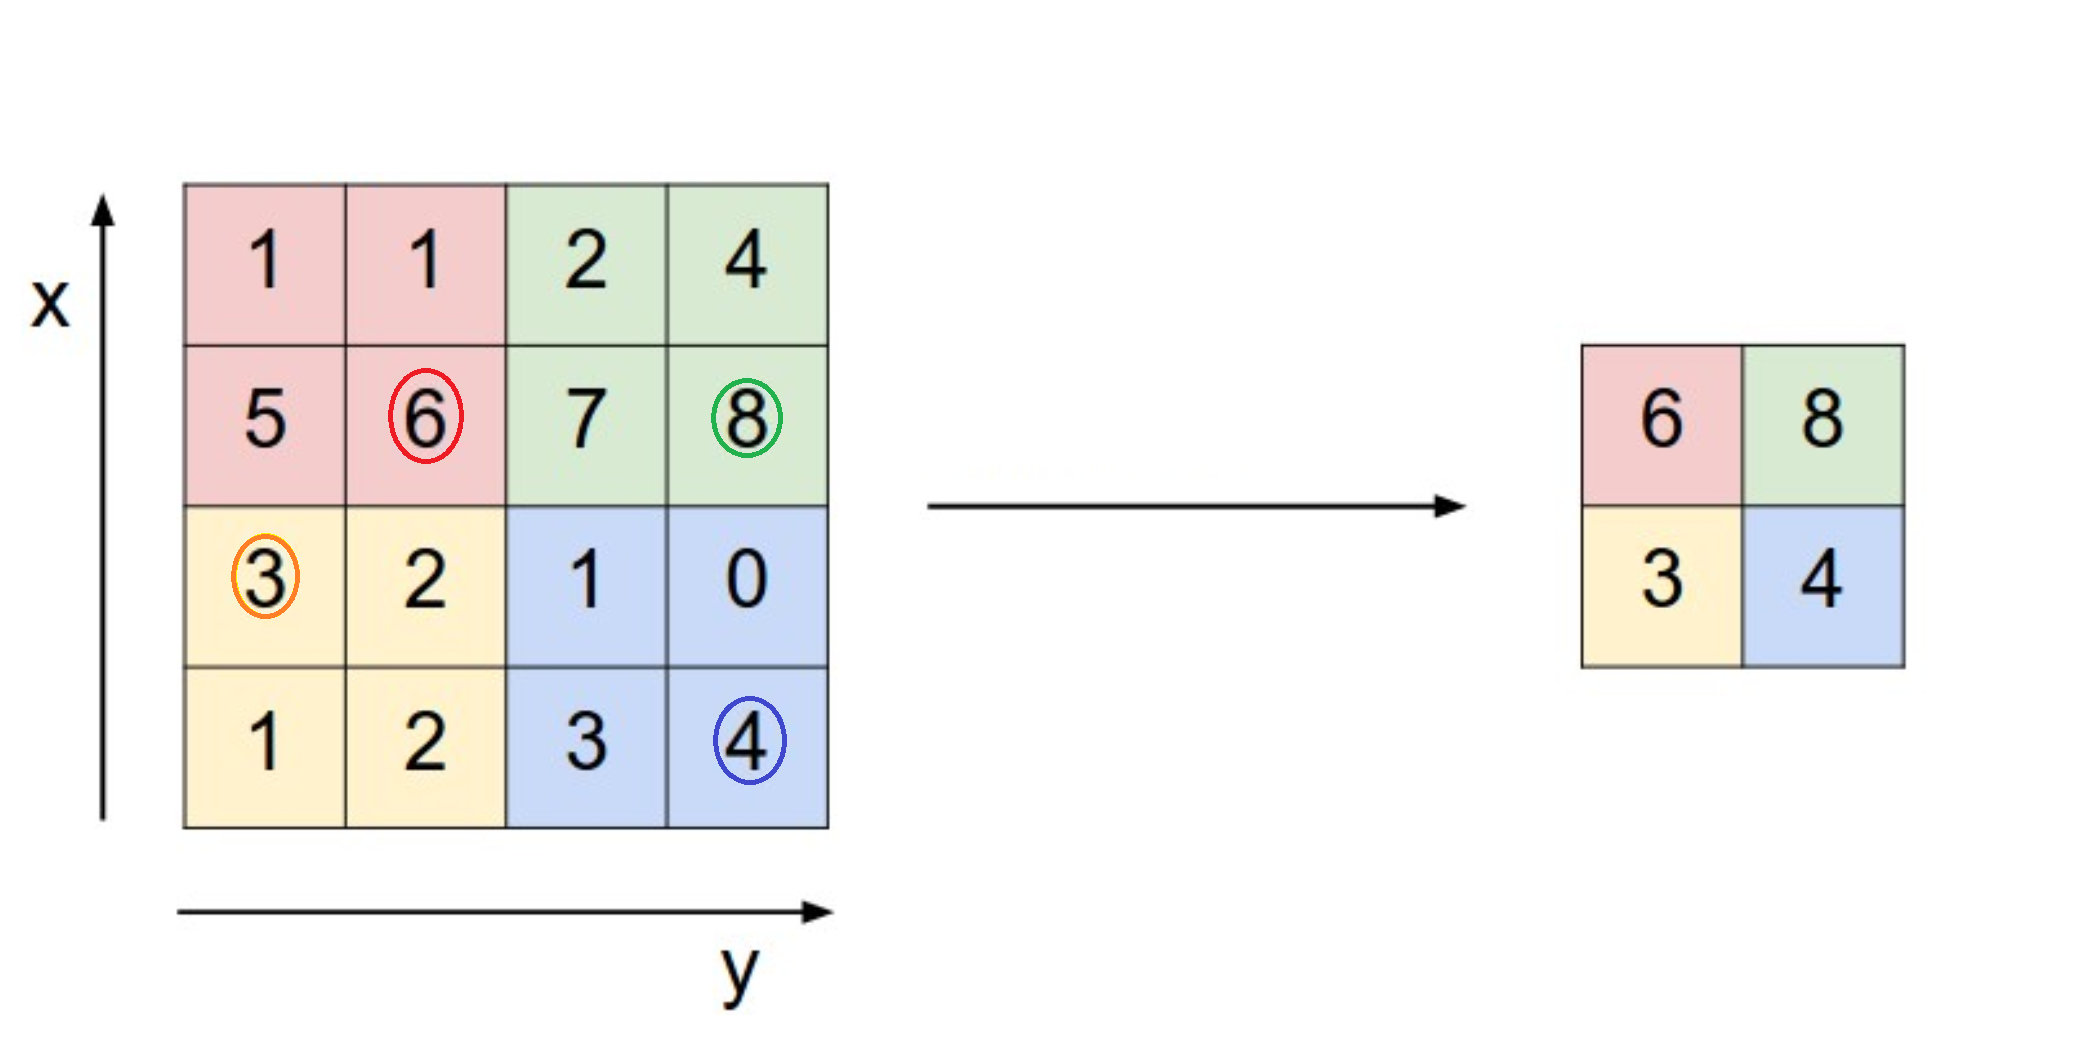
\includegraphics[scale=0.3]{pooling.png}
\caption{Pooling mit stride = 2}
\end{figure}

\item \textbf{4. Fully Connected Layer} Diese Neuronen-Schicht soll die Ausgabe nach den oben genannten Schritten interpretierbar machen und auf Klassen-Scores abbilden. Jedes Neuron ist mit jedem aktivierten Gewicht davor liegenden Schicht verbunden.
\begin{figure}[h]
\centering
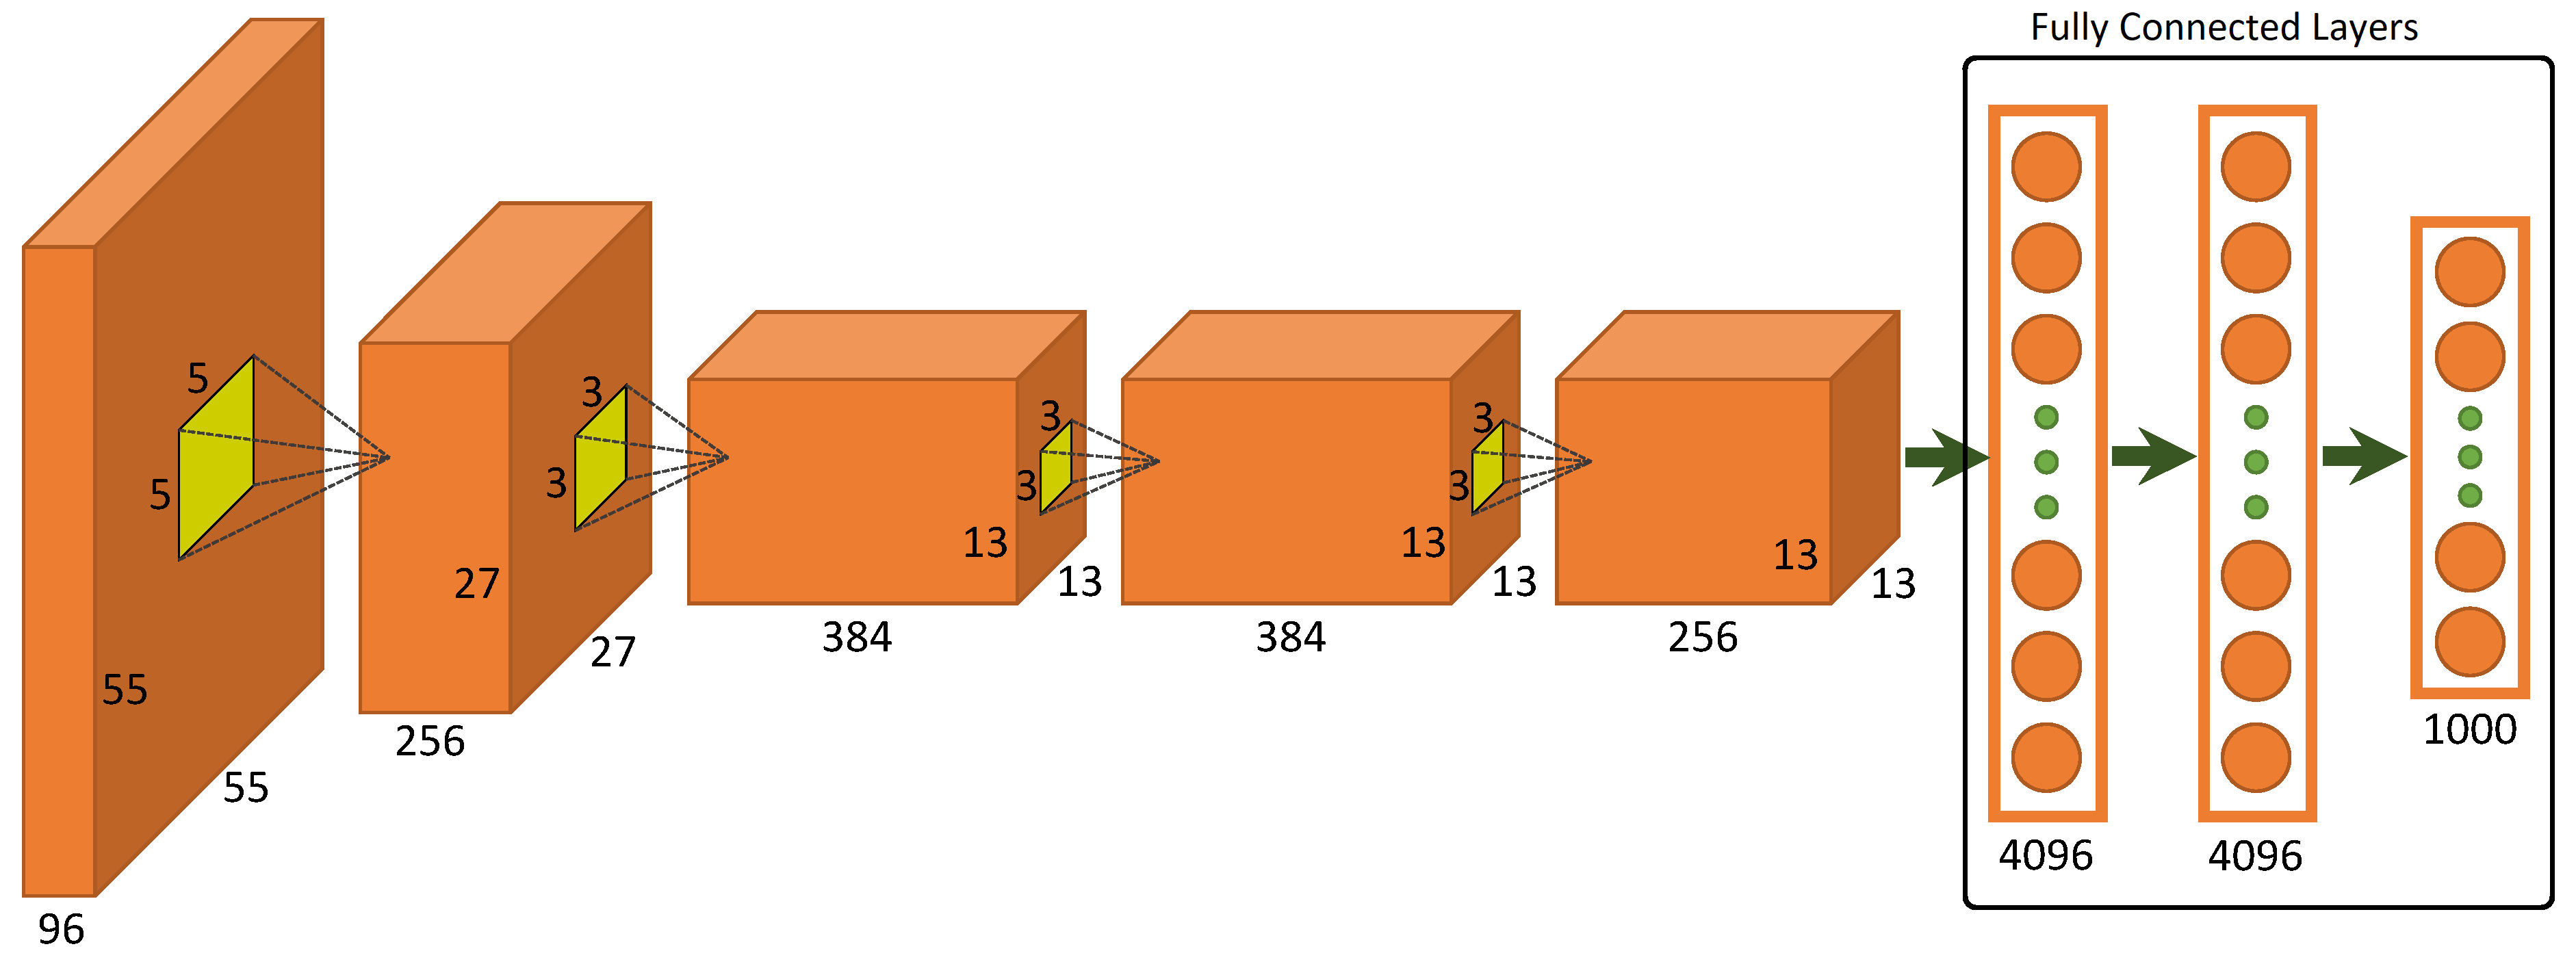
\includegraphics[scale=0.2]{conv-construction.png}
\caption{Gewöhnliches Convnet mit Fully-Connected-Layers zum Schluss}
\end{figure}

\end{itemize}

\begin{figure}[h]
\centering
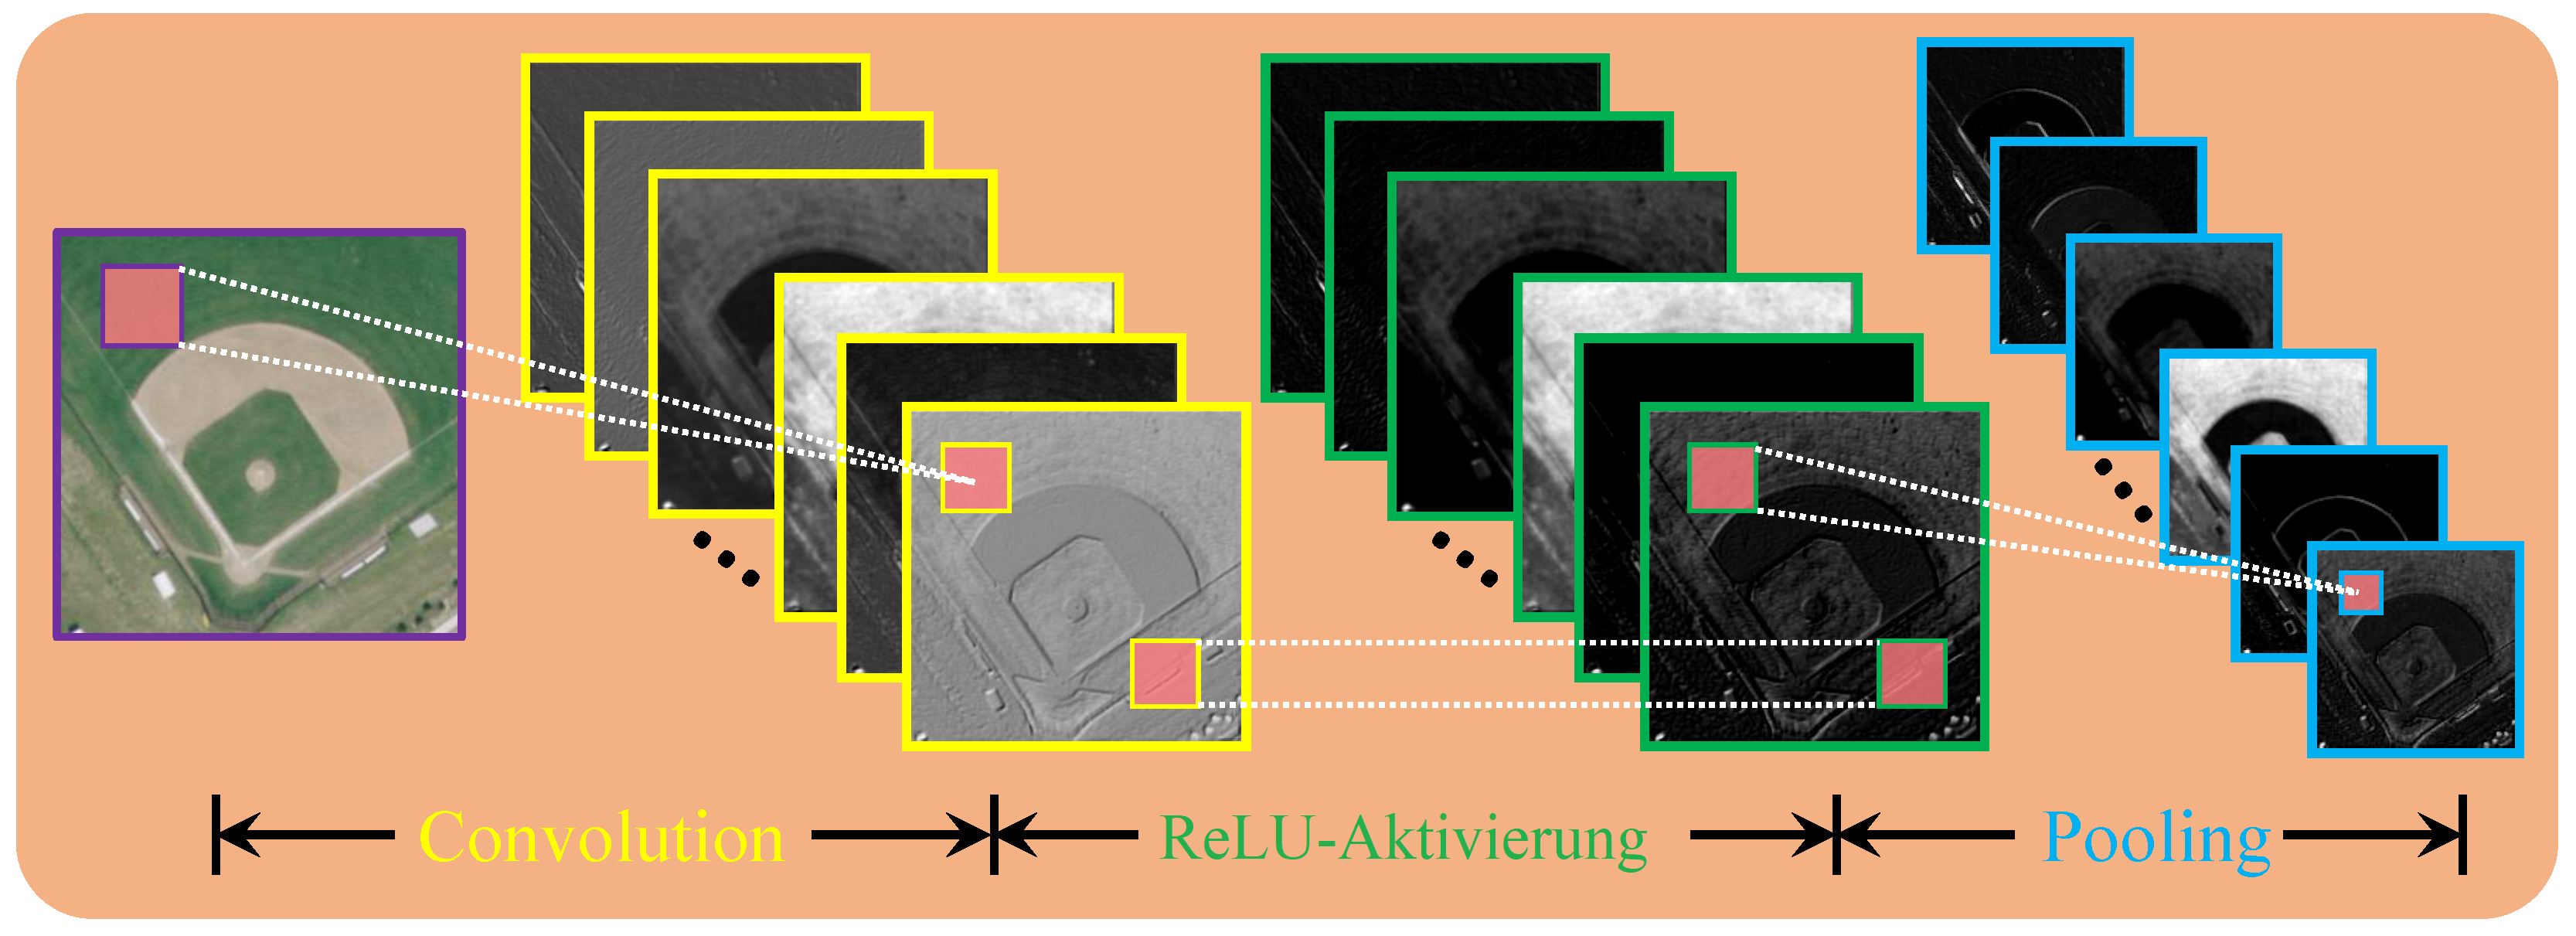
\includegraphics[scale=0.7]{conv-layers.png}
\caption{Verbildlichung der Schritte 1-3 durch Anwendung von Convolution auf ein Luftbild\protect\footnotemark}
\end{figure}
\footnotetext{http://www.mdpi.com/2072-4292/7/11/14680/htm}


\subsection{Recurrent Neural Network}
Ein Recurrent Neural Network (RNN) ist ein zeitabhängiges neuronales Netz, mit welchem sich Zustände vorhersagen lassen. So lassen sich mit einem RNN z.B. folgende Probleme Lösen:

\begin{itemize}
\item Image Captioning
\item Sentimentanalyse (Stimmungserkennung im Text Mining)
\item Sprachübersetzung, Textproduktion und Vorhersage von Worten
\item Videoklassifikatio
\item Vorhersage von geologischen Aktivitäten
\end{itemize}

Ein Zustand $h_t$ und eine Ausgabe $y_t$ eines RNN zu einem bestimmten Zeitpunkt $t$ berechnet sich wie folgt:

\[h_t = f(W_{xh} x_t + W_{hh} h_{t-1} + b1)\]
\[y_t = g(W_{hy} h_t + b2)\]

Hierbei enthalten die Gewichtsmatritzen $W_{xh}$, $W_{hh}$, $W_{hy}$ die zu lernenden Parameter zwischen Input Layer, Hidden Layer und Output Layer. Die Funktionen $f$ und $g$ sind Nichtlinearitäten.

\textbf{Beispiel:}\\
Ein RNN wird mit einer gegebenen Sequenz ('h' 'e' 'l' 'l' 'o') 
trainiert, so dass es bei der Eingabesequenz x = ('h' 'e' 'l' 'l') die Sequenz ('e' 'l' 'l' 'o') und somit den Buchstaben 'o' korrekt vorhersagt. 
\begin{figure}[h]
\centering
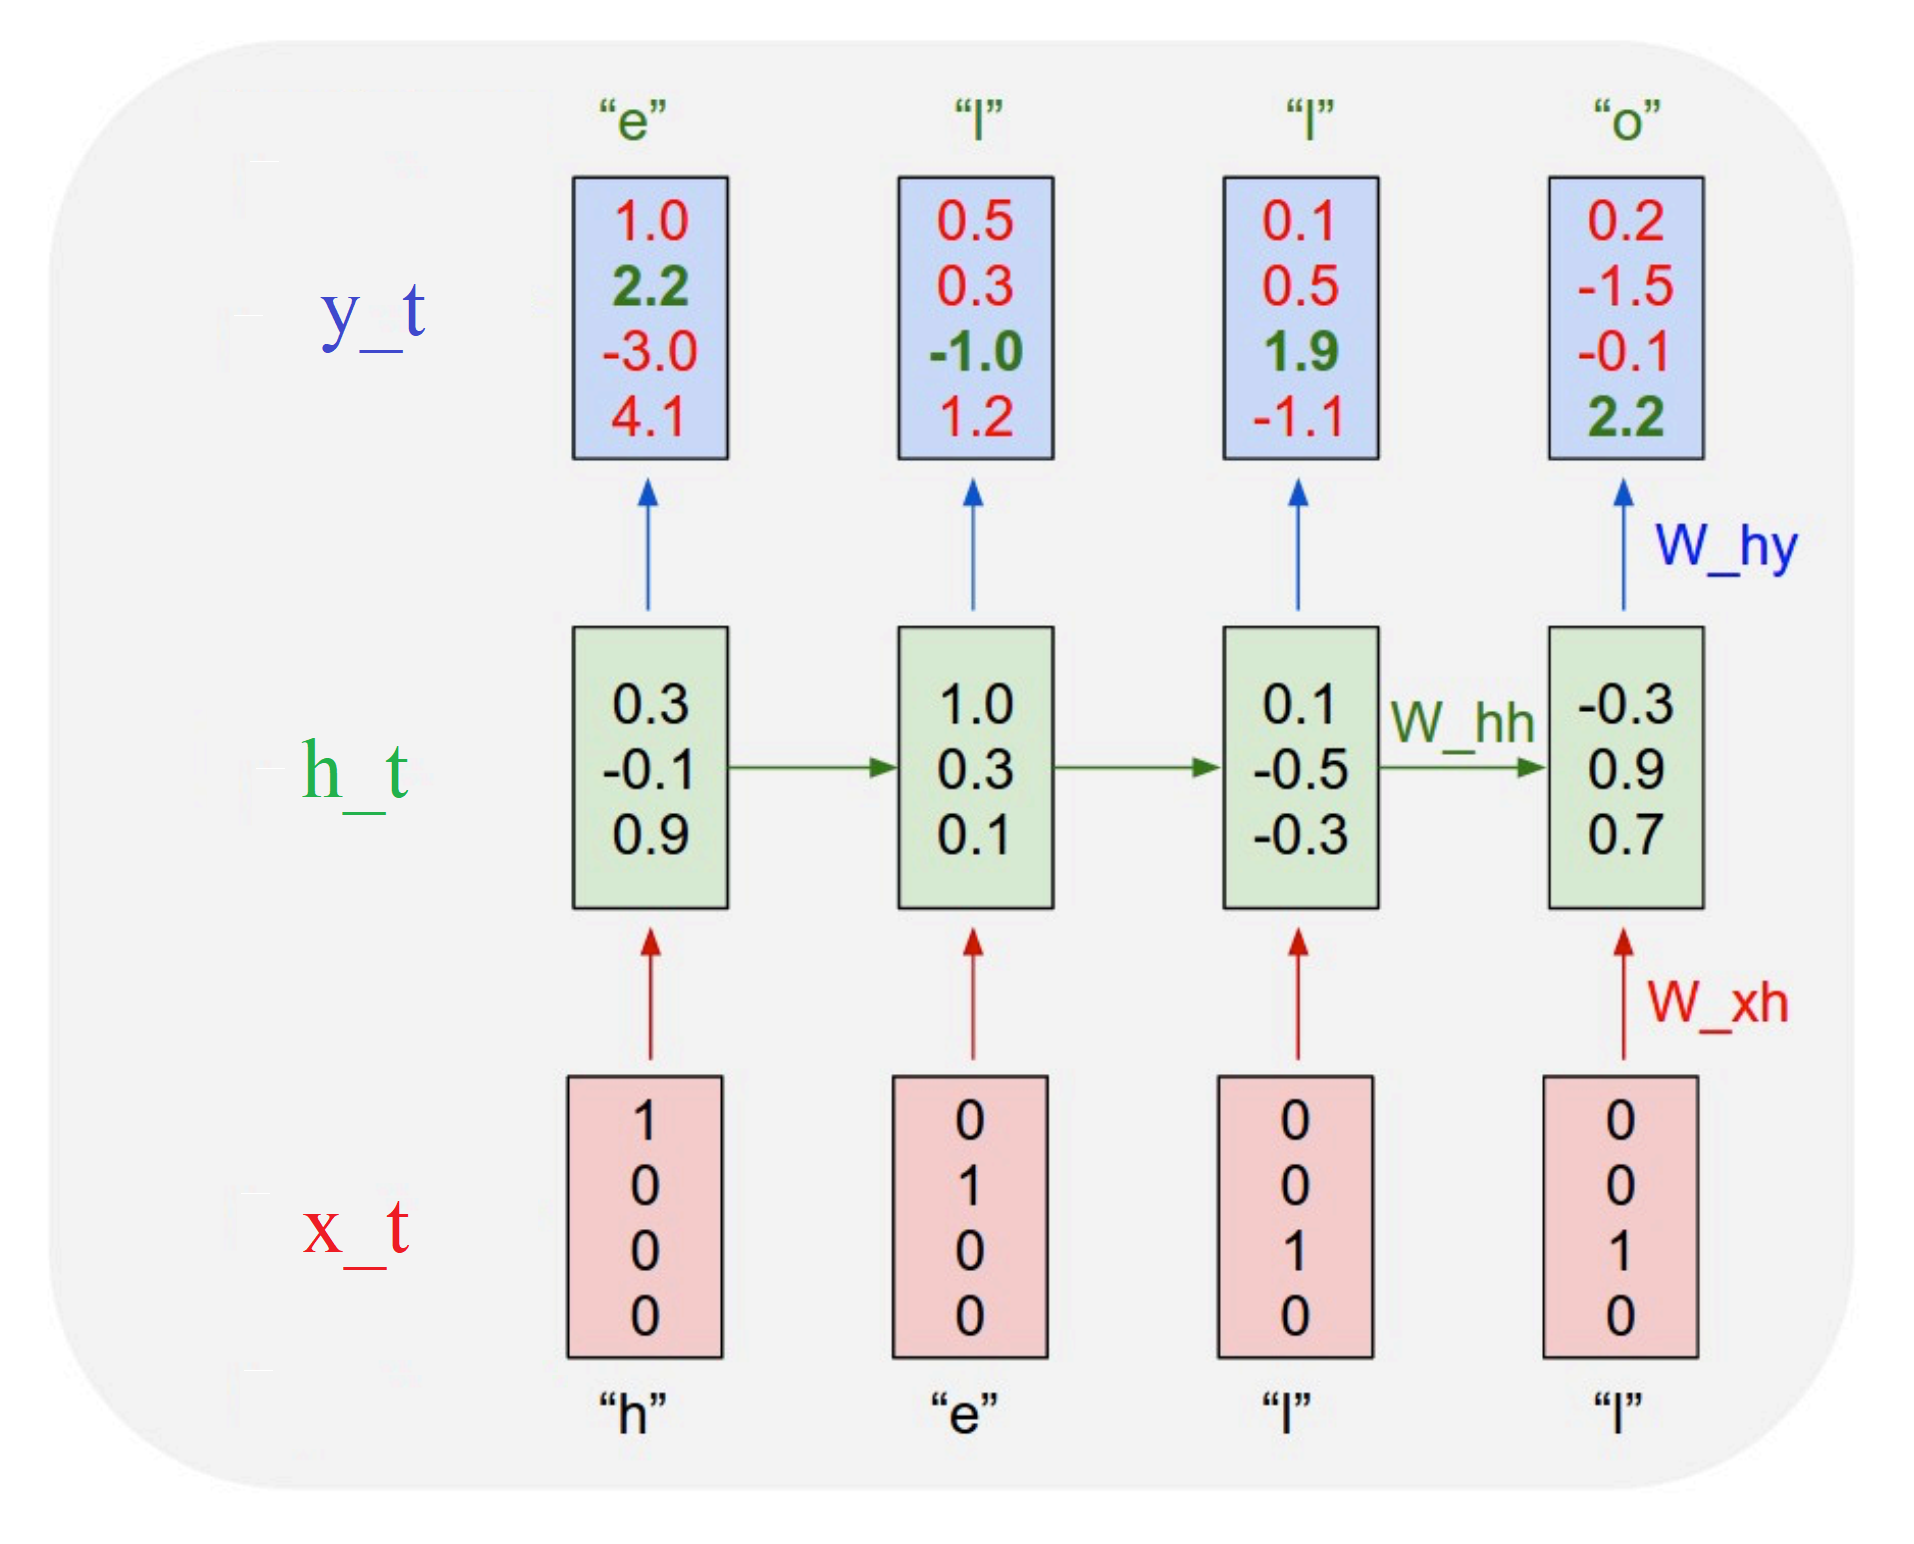
\includegraphics[scale=0.35]{RNN.png}
\caption{RNN vervollständigt das Wort \textit{hello}}
\end{figure}

Die Gewichtsmatrix $W_{xh}$ speichert, wie Buchstaben zu Hidden States umgewandelt und inkrementiert werden. $W_{hy}$ lernt, welcher Ausgabebuchstabe zu gegebenem Hidden State passt und die Matrix $W_{hh}$ akkumuliert und migriert alle bisherigen Eingaben im zeitlichen Verlauf zu einem gemeinsamen Hidden State.

\subsection{Long Short Term Memory Netzwerke}

\textbf{Das Problem der Langzeitabhängigkeit}























\newpage
\section{Machine Learning in Geowissenschaften}

\subsection{Herausforderungen und Chancen von Machine Learning \cite{machgeo}}
\textbf{Einleitung}\\
Die moderne Geowissenschaft steht vor vielen Herausforderungen, wie den Prognosen zu Klimawandel, Luftverschmutzung, Naturkatastrophen, Ressourcenverbrauch oder den Risiken für Erdbeben, Landrutsch und Vulkanausbrüchen. Die Forschung an solchen Problemen macht die interdisziplinäre Arbeit sämtlicher Wissenschaften unumgänglich.
Geowissenschaften haben sich in den letzten Jahrzehnten  zu einer Big-Data Disziplin entwickelt. Angestoßen wurde diese Entwicklung durch sämtliche technologische Verbesserungen, wie dem Wachstum der Computerleistung. Aufwändige Simulationen und die Demokratisierung von Datenbeständen, deren öffentliche Verbreitung im Internet und vielseitige Beteiligungsmöglichkeiten trugen ebenfalls dazu bei. Die wachsende Verbreitung großer geowissenschaftlicher Datenbestände ermöglicht ein enormes Potenzial für Maschinelles Lernen.\\

\bigskip

\textbf{Sammeln von Geodaten}\\
Die Erde ist ein komplexes dynamisches System, bestehend aus Litosphäre, Biosphäre, Atmosphäre, Hydrosphäre. Einzelne Bestandteile dieses Systems (z.B. Ozeanschichten oder die Bodenbedeckung) befinden sich in einem ständigen Wandel und interagieren miteinander. Um Daten solcher Phänomene zu erheben, gibt es vor allem zwei Möglichkeiten:
\begin{itemize}
\item Messen mithilfe von Sensoren in/auf Satelliten, Flugzeugen, Ballons, Drohnen, Wetterstationen, Schiffen, Bojen.\newline
Sensorbasierte geowissenschaftliche Beobachtungen sind nicht uniform gerastert und beziehen sich häufig auf irreguläre Zeitintervalle (zum Beispiel schwankt die Position einer Boje mit der Zeit). Sie eignen sich jedoch Hervorragend zum sammeln von Daten wie Oberflächentemperatur, Luftfeuchtigkeit, Reflektionintensität, Chemischer Zusammensetzung der Atmosphäre, Strömungen und Drücke, Emissionen, seismischer Aktivität und der Oberflächengestalt der Erde. Diese Vielfalt an geologischen Eigenschaften erfordert bezüglich eines gegebenen Problems eine individuelle Zusammenstellung von relevanten Datensätzen. Die Datentypen müssen gegebenenfalls konvertiert und die Datenbestände interpoliert werden, um sie besser interpretierbar zu machen.

\item \textbf{Ableiten aus mathematischen Modellen und Simulationen}
Geologische Prozesse, ihre Interaktionen und Änderungen sind auf physikalische Gesetze zurückzuführen. Zum Beispiel sind Bewegungen von Wasser in der Liosphäre auf die Strömungsdynamic zurückzuführen. Ein Nachteil physikalischer Berechnungen auf Grundlage von Modellen für komplexe Systeme ist leider deren Ungenauigkeit. Dennoch eignen sie sich zur näherungsweisen Darstellung des zeitlichen Verlaufes von geophysikalischen Phänomenen. Ein weiterer Vorteil ist, dass Simulationen besonders große Datensätze erzeugen können, wenn Daten für große Zeitintervalle von Interesse sind. Diese ermöglichen dann wiederum eine Datenbasierte Analyse mittels Machine Learning.
\end{itemize}
\bigskip
\textbf{Herausforderungen}
Leider ist die Nützlichkeit von Machine Learning für Knowledge Discovery häufig begrenzt. Geophysikalische Objekte sind häufig nicht klar definiert (keine klar definierten Grenzen) und ändern sich häufig. Daten zu solchen Objekten können ebenfalls unterschiedliche Auflösungen haben, rauschen, unvollständig oder ungenau sein. Auch kann die zeitliche Auflösung aus historischen Gründen stark variieren (z.B. ein Weltkrieg, in dem historische Datensätze zerstört wurden). Auch liegen häufig nicht ausreichend Geländedaten vor. Die Herausforderungen lassen sich in 3 Hauptkategorien unterteilen:

\begin{itemize}
\item \textbf{Eigenschaften Geologischer Prozesse}
\begin{itemize}\item \textbf{Amorphe Grenzen (Wellen, Flüsse, Stürme)} Segmentierungs- und Clusteringverfahren sowie Maßnahmen für Feature-Charakterisierungen sind notwendig.
\item \textbf{Raumzeitliche Struktur}  
Für viele Machine Learning Methoden nimmt man an, dass beobachtete geophysikalische Eigenschaften nicht korrelieren und die erhobenen Daten gleichverteilt sind. Die Realität sieht anders aus. 
Benachbarte Orte sind stark korreliert (Wahrscheinlichkeit für Grasland ist in der Nähe eines Waldes größer als in einer Wüste). Änderungen (Wald => Wüste) bewirken Zustände, die für eine unbestimmbare Zeit persistieren (Die Wüste wird nicht regelmäßig zum Wald und umgekehrt), was auf Klimaveränderungen zurückzuführen ist.
Zwei weit entfernte Orte können ebenfalls stark korrelierte Eigenschaften besitzen (z.B. Temperatur, Druck). Man nennt diese meist meteorologischen Korrelationen Telekonnektionen .
\item \textbf{Hochdimensionalität} Die Erde ist eines der komplexesten bekannten Systeme mit einer extrem großen Anzahl an Variablen, die alle miteinander in sowohl räumlich als auch zeitlich relativ zur Größe der Erde winzigen Skalen miteinander wechselwirken. Für eine Verarbeitung und Speicherung von Daten solcher Systeme ist die Rechenleistung heutiger Computer nicht ausreichend.
\item \textbf{Raumzeitliche Variabilität} Geologische Prozesse können stark schwanken, sowohl in kurzen Zeitintervallen (Jahreszeiten, Tidenhub), in langen Zeitintervallen (Polsprung, Präzession, Klimawandel) als auch räumlich (Gebirgsformationen, Vegetationszonen, Klimazonen). Es ist sehr schwierig ein Modell zu trainieren, dass alle diese Prozesse vereint. Eine lokale und zeitliche Begrenzung der Datensätze ist zwingend erforderlich.
\item Seltene Phänomene - Seltene Ereignisse wie z.B. Vulkanausbrüche, Tsunamis und Erdbeben verfälschen das Modell, da sie nur für ein Training auf viel größeren Zeitskalen geeignet sind. Aus diesem Grund müssen sie erkannt und aus dem Modell herausgerechnet werden. Dies ist nahezu unmöglich, da es hierzu keine ausreichenden Erfahrungswerte gibt.
\end{itemize}

\item \textbf{Sammeln von Geodaten}
\begin{itemize}
\item Daten mit verschiedenen Auflösungen - Beispiel: Zur Beurteilung von Waldbränden müssen Bilder aus Luftaufnahmen und Satellitenbilder miteinander kombiniert werden. Die Flugzeugbilder haben eine höhere räumliche Auflösung, die Satellitenbilder wurden jedoch in regelmäßigen Zeitabständen aufgenommen. Aus diesem Grund müssen Interpolations- oder Upsamplingmethoden entworfen werden, um die beiden Arten von Bildern vergleichbar zu machen.
\item Rauschen, Unvollständigkeit, Ungenauigkeit - Viele Geodatensätze sind unvollständig oder rauschen, weil z.B. Sensoren temporär ausgefallen sind oder unter verschiedenen Wetterbedingungen Messungen durchgeführt haben. Manche Daten sind erst dann interpretierbar, wenn Sie mit einem mathematischen Modell kombiniert werden. Dieses kann die Interpretierbarkeit jedoch ebenfalls beeinflussen.
\end{itemize}

\item \textbf{Mangelhafte Datensätze}
\begin{itemize}
\item \textbf{Kleine Sample-Größe} Viele Datenbestände sind niedrigfrequent und extrem ungenau, wenn sie aus einer Zeit stammen, in welcher es entweder keine oder nur wenige Messinstrumente gab. Auch gibt es Orte, an denen es nur schwer möglich ist (zeitlich hochfrequente) Messungen durchzuführen (Bohrkernanalyse in Antarktis o.ä., Bäume mit ausreichendem Alter für Jahresringe). Eisbohrkerne aus der Antarktis lassen zudem keine Rückschlüsse über die Klimatischen Verhältnisse in anderen Regionen zu. 
\item  \textbf{Mangelhafte gelabelte Geländedaten} Oft liegen Geländedaten in mangelnder Qualität vor. Dies liegt daran, dass sie nur mit Zeit- und Kostenintensiven Maßnahmen zu beschaffen sind. Eine geringe Datenqualität führt zu einem langsamen Trainingsprozesses und zu Unter- oder Überanpassung des Modells, was die Aussagekraft stark einschränkt.
\end{itemize}
Aus beiden oben genannten Gründen müssen Trainingsmodelle entwickelt werden, die mit kleineren Datensätzen zurecht kommen.
\end{itemize}
\bigskip
Maschinelles Lernalgorithmen können dazu beitragen, Geowissenschaftliche Objekte und Ereignisse zu Charakterisieren und somit helfen, das Erdsystem besser zu verstehen. Während traditionelle Ansätze auf handgefertigten Algorithmen basieren, können Machine Learning Algorithmen mit ihrer automatischen Mustererkennung die Berechnungszeit deutlich verkürzen. Eine große Herausforderung stellt die Charakterisierung von physikalisch ungenau definierten Objekten dar. Unsupervised Learning kann dabei helfen, anomalische Objekte aufzuspüren (z.B. Landminen).\\
\bigskip
Ein weiterer großer Vorteil von Machine Learning ist die Erzeugung von Geodaten aus nur schwer beobachtbaren Prozessen (z.B. Methanausstoß und Konzentration in der Atmosphäre). Supervised Learning kann verwendet werden, um Fernerkundungsdaten zu analysieren und daraus Aussagen über das Ökosystem abzuleiten (z.B. Gesundheit der Vegetation oder Wasserqualität). Eine besondere Herausforderung ist dabei die Heterogenität solcher Daten, wie bereits weiter oben beschrieben. Eine mögliche Lösung sind Multi-Task-Learning-Frameworks, welche Datensätze zuerst in homogene Partitionen unterteilen (hierarchisches Clustern), und dann auf jeder dieser Partitionen einzeln trainieren. Dieses Vorgehen ist eine Regularisierungstechnik, welche die Überanpassung des Modells verhindern soll. Folgende Abbildung zeigt die Verbesserung der Genauigkeit der geschätzten Waldbedeckung vier brasilianischer Staaten, wobei die rot markierten Bereiche die Residuen darstellen.
\begin{figure}[h]
\centering
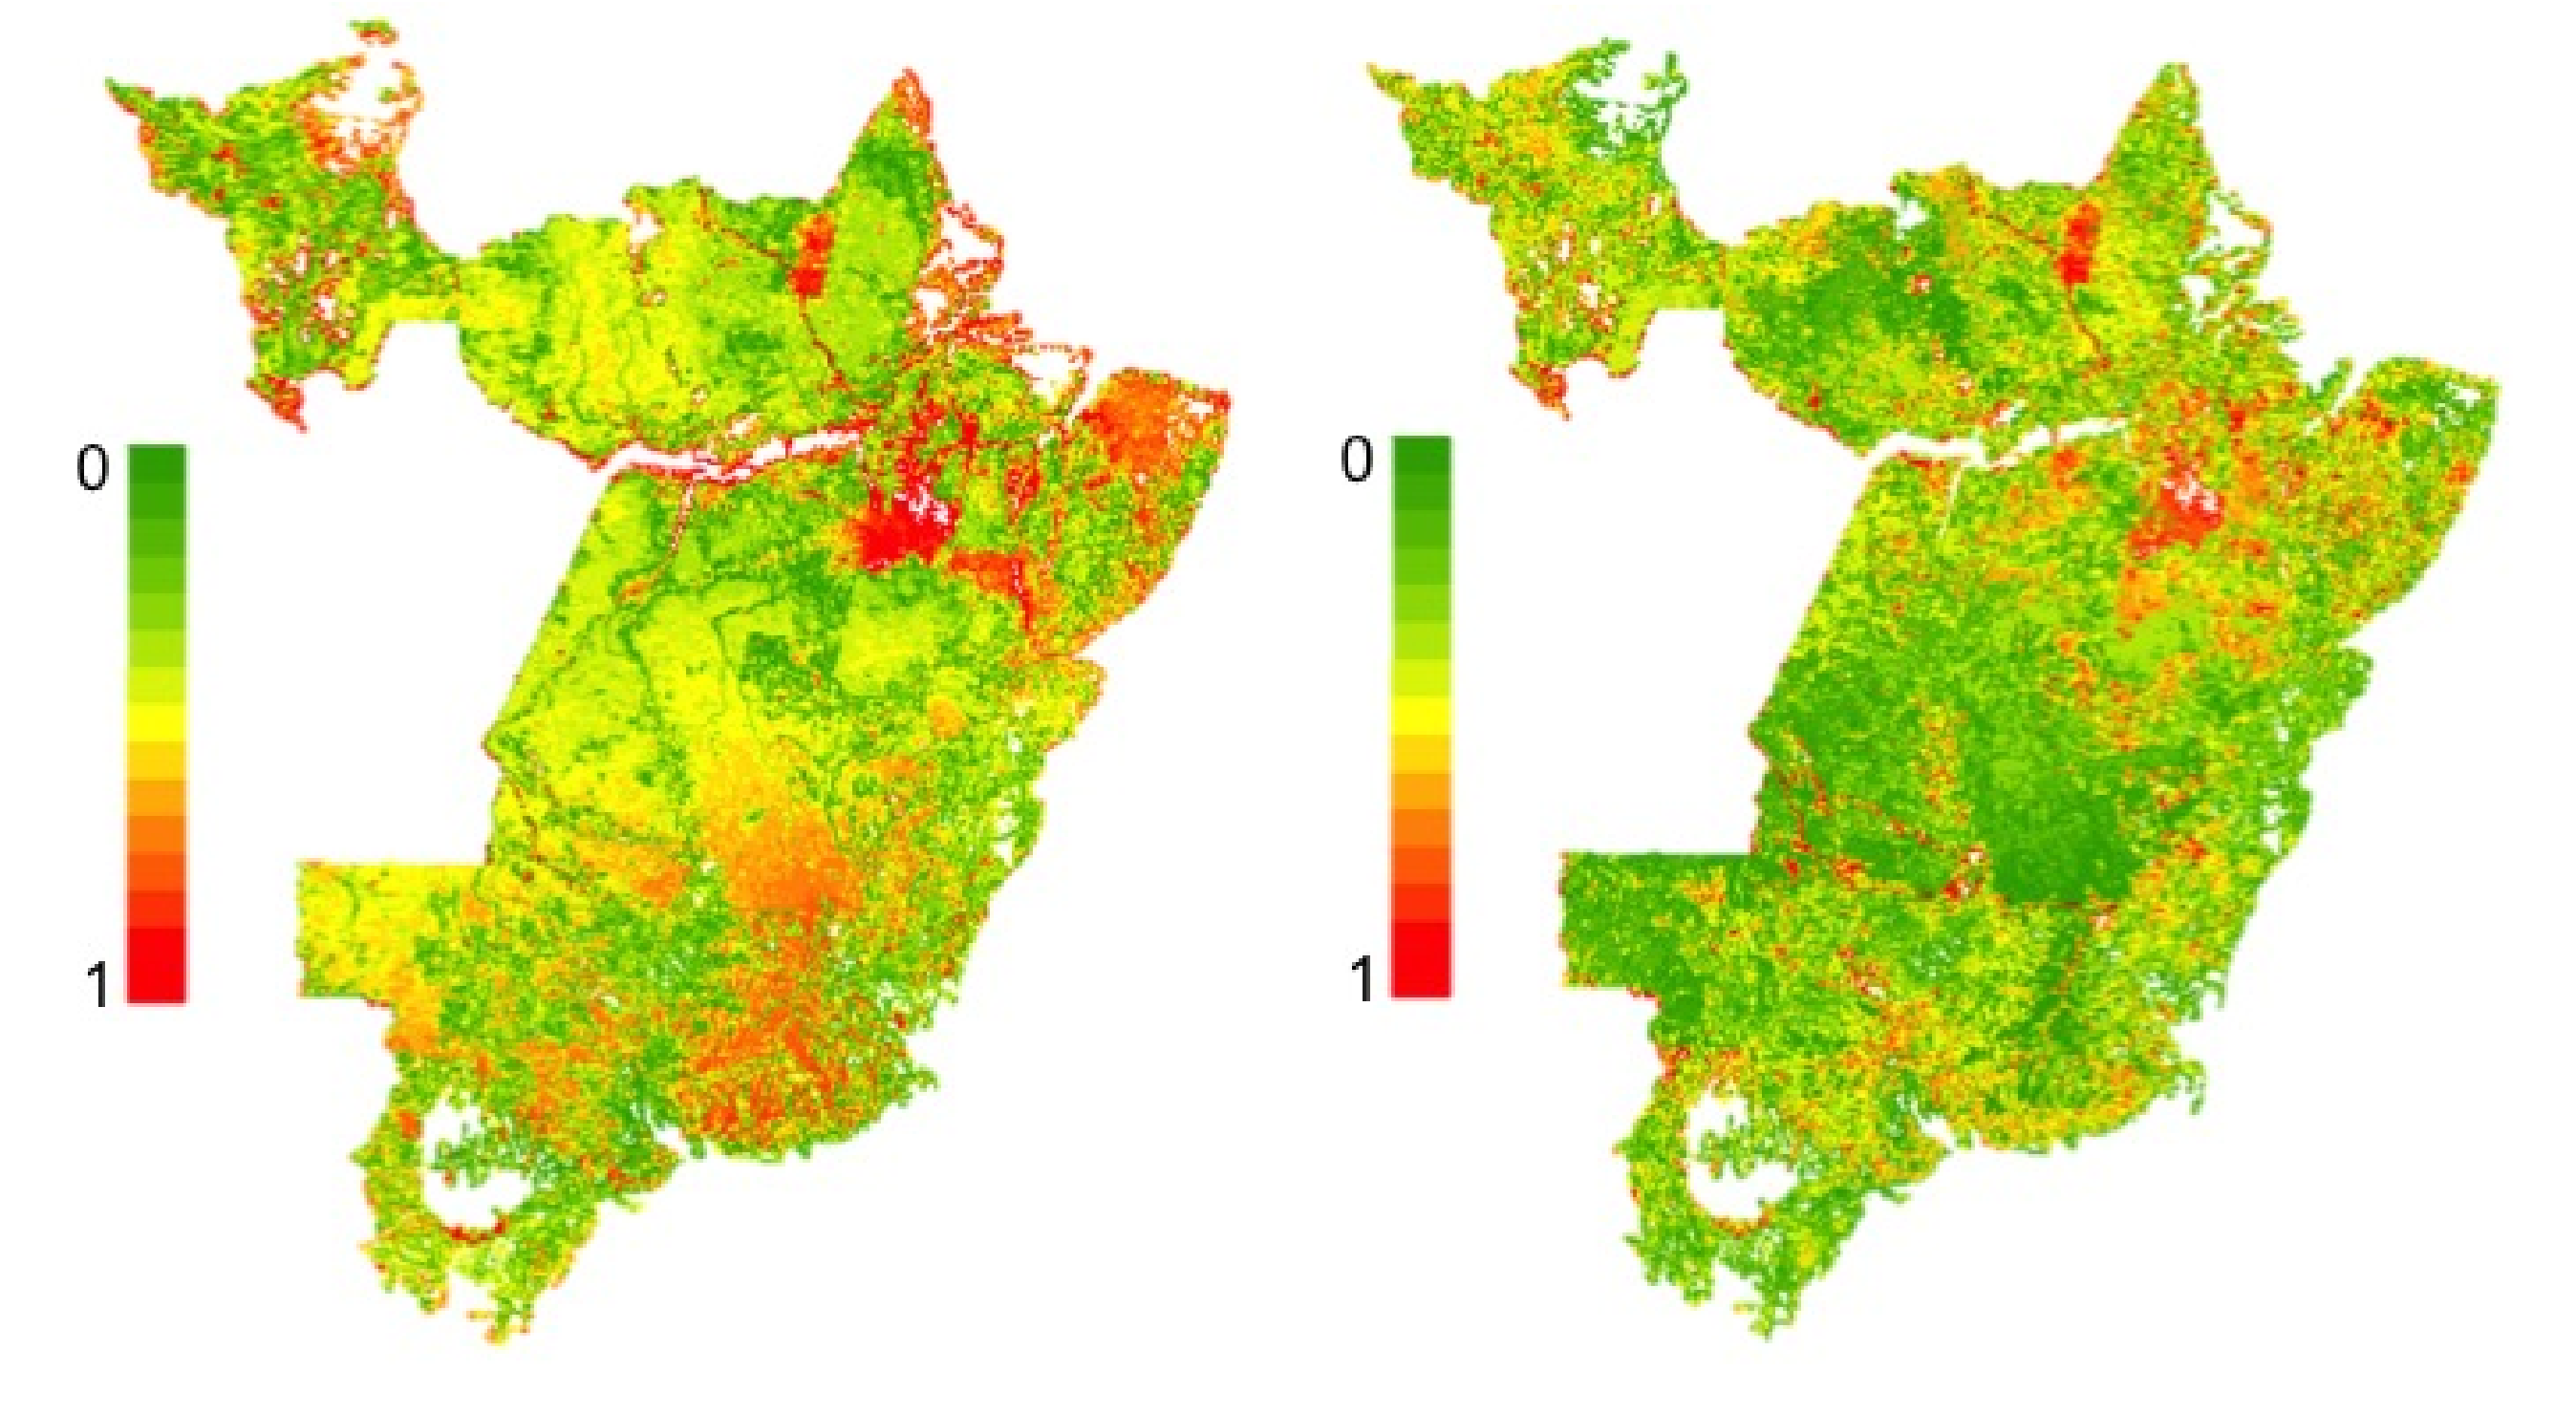
\includegraphics[scale=0.25]{multi-task-learning.png}
\caption{Schätzung der Waldbedeckung in Brasilien \protect\footnotemark}
\end{figure}
\footnotetext{A. Karpatne, Z. Jiang, R. R. Vatsavai, S. Shekhar, and V. Kumar,
Monitoring Land-Cover Changes. IEEE Geoscience and Remote
Sensing Magazine, 2016}\\
\bigskip
\textbf{Nichtstationarität, Heterogenität und Mangeldaten}\\
Zum Umgang mit der Nichtstationarität (= Variable folgt keinem konstanten Wert) von Klimadaten wurden lernende Algorithmen entworfen, welche die Vorhersagen verschiedener Klimamodelle kombinieren. Statt eines Mittelwertes über die Klimamodelle berücksichtigt der selbstlernende Algorithmus zusätzlich  die nichtstationären Dateneigenschaften und erzeugt wesentlich genauerer Vorhersagen.

Heterogene und minderqualitative Daten können mithilfe von \textit{Adaptive Ensemble Learning} und \textit{Label Refinement} besser analysiert werden.

Zur Näherung von Geophysikalischen Variablen mit Daten geringer zeitlicher Auflösung und fehlender Labels können folgende Techniken verwendet werden:
- Regularisierer (für zeitl. Auflösung)
- Semi-Supervised-Learning (fehlende Labels)
- Active Learning (genauere Ergebnisse für Berechnungsprobleme)
- Unsupervised Learning (bessere Näherung für geophysikalische Größen und Kartierung von Flächenänderungen durch z.B. Insektensterben, Waldabholzung und Ackerlandumwandlung)\\

\bigskip
\textbf{Techniken für Langzeitvorhersagen}\\
Eine Möglichkeit für Langzeitvorhersagen war bisher die Verwendung von physikalischen Modellsimulationen. Diese können jedoch auch als Zeitreihen-Regressions-Problem aufgefasst werden. Mögliche Methoden zur Lösung solcher Probleme sind z.B.:
\begin{itemize}
\item Exponential Smoothing Techniques
\item Autoregressive Integrated Moving Average (ARIMA) Modelle
\item State-space Modelle 
\item Hidden Markov Modelle
\item Kalman Filter
\end{itemize}
Transfer Learning - Ein zu trainierendes Modell für ein Problem mit wenig Daten soll mithilfe eines zuvor trainierten Modells mit vielen Daten das Problem besser lösen.\\

\bigskip
\textbf{Relationen und Kausalität}\\
Geophysikalische Zusammenhänge (z.B. Telekonnektionen und Dipole), sollen sich mithilfe datenbasierter Ansätze besser verstehen lassen. Man erhofft sich durch sie die Entdeckung neuer Korrelationsmuster.
Darüber hinaus können graphenbasierte Repräsentationen von Klimadaten mithilfe von Clustering und Mustererkennung besser analysiert werden.
\bigskip
Eine besondere Herausforderung bei der Korellationserkennung ist der besonders große Suchraum mit all seinen raumzeitlichen Objekten und dynamischen, rauschenden und unvollständigen Geodaten. Es herrscht ein großer Bedarf an neuen Ansätzen, die gleichzeitig sowohl Zusammenhänge als auch die dazugehörigen interagierenden Objekte erkennen.\\
Ursache-Wirkungszusammenhänge zu entdecken ist eine weitere wichtige Aufgabe in den Geowissenschaften. Ein häufig eingesetztes Tool für die Analyse von solchen kausalen Zusammenhängen ist die multivariate Grangeranalyse mittels Vektorautoregression. Auf diese Weise können z.B. Sturmverläufe vorhergesagt werden. Weitere kaum erforschte Mgölichkeiten sind das Reinforcement Learning und stoastische Anstze der dynamischen Programmierung zur Lösung von Entscheidungsproblemen.
\\ \bigskip
\textbf{Deep Learning}\\
Neuronale Netze haben die Eigenschaft, komplexe Features mithilfe der Verknüpfung weniger komplexer Features darzustellen. In Kombination mit dem Training großer Datensätze und der Fähigkeit, Fehler an den Nodes der Hidden-Layers zu minimieren, haben neuronale Netze weite Felder im Bereich Machine Learning revolutioniert. Darunter auch  Supervised, Semi-Supervised, und Reinforcement Learning. Häufig werden neuronale Netze eingesetzt, wenn es schwierig ist, mittels handgeschriebener Algorithmen die wirklich relevanten Features aus einem komplexen Datensatz (wie es auch Geodatensätze sind) zu extrahieren. Geophysikalische Fragestellungen und Probleme haben viele Ähnlichkeiten zu den Themen, die im Bereich Computer Vision und Spracherkennung behandelt werden. \\
\bigskip
Während man ein Convolutional Neural Network einsetzt, um auf einem Bild eine Katze zu klassifizieren, kann man dieses auch verwenden, um Wetterphänomene wie Tornados auf Satellitenbildern zu erkennen. \\ \bigskip
Rekurrente Neuronale Netze mit Longshort-Term-Memory Zellen (LSTM) können z.B. genutzt werden, um zeitlich dynamische Plantagen mittels Fernerkundungsdaten kartografieren. RNNs besitzen die Eigenschaft besitzen, zeitlich vergangene Information zu speichern und in zukünftige Vorhersagen mit einzubeziehen. Aus diesem Grund eignen Sie sich zur Vorhersage von geologischen Ereignissen mit angemessener Vorlaufzeit.\\
\bigskip
Deep Learning kann bisher nur bei ausreichend gelabelten Daten zum Einsatz kommen. Aus diesem Grund herrscht hier ein Bedarf an neuen Verfahren, die mit nur wenigen Daten zurechtkommen.\\
\bigskip
\textbf{Fazit}\\
Die Forschung der letzten Jahre hat gezeigt, dass weder ein reiner Datenansatz noch ein reiner mathematischer Modellansatz ausreichend ist, um Knowledge Discovery effizient betreiben zu können. Aus diesem Grund sollten zukünftige physikalische Erkenntnisse möglichst früh und tief in Datenwissenschaftlichen Ansätze einbezogen werden. Auf diese Weise lässt sich auch die Wahrscheinlichkeit für Overfitting reduzieren, vor allem bei mangelnden Trainingsdaten.

\subsection{Beispiele}

\section{Tensorflow}
\section{Erstes eigenes CNN}

%----------------------------------------------------------------------------------------
%	CHAPTER 3
%----------------------------------------------------------------------------------------

\chapter{Clusteringverfahren}
\section{Probabilistisches und Possibilistisches Clustering}
\subsection{FCM und PFCM}
\subsection{Vorraussetzungen für die Anwendung auf Geodaten}
\subsection{Eigener Algoritmus (noch ohne Name)}
\section{CVI}
\subsection{NPC}
\subsection{FHV}
\subsection{Otsu-Binarisierung}
\subsection{VAT-Algorithmus}
\section{Clustering auf unvollständigen Daten}

%----------------------------------------------------------------------------------------
%	CHAPTER 4
%----------------------------------------------------------------------------------------

\chapter{Fazit und Ausblick}
\section{Ausblick - Mein Thema für die Masterarbeit}

\printbibliography

\vfill
\end{document}